

\documentclass[titlepage, a4paper]{article}
\usepackage[swedish]{babel}
\usepackage[utf8]{inputenc}
\usepackage{color}
\usepackage{graphicx}
\usepackage{etoolbox}

% Sidformat
\usepackage{a4wide}

% Fixa Appendix-titlar
\usepackage[titletoc,title]{appendix}

% Bättre bildtexter
\usepackage[margin=10pt,font=small,labelfont=bf,labelsep=endash]{caption}

% Enkelt kommando som låter mig attgöra-markera text
\newcommand{\todo}[1] {\textbf{\textcolor{red}{#1}}}

%% Headers och Footers
\usepackage{fancyhdr}
\pagestyle{fancy}
\lhead{\includegraphics[scale=0.12]{../logga/Logga1.png}}
\rhead{\today}
\lfoot{\LIPSkursnamn \\ \LIPSdokumenttyp}
\cfoot{\thepage}
\rfoot{\LIPSprojektgrupp \\ \LIPSprojektnamn}

%% Titelsida
\newcommand{\LIPSTitelsida}{%
{\ }\vspace{45mm}
\begin{center}
  \textbf{\Huge \LIPSdokument}
\end{center}
\begin{center}
  {\Large Redaktör: \LIPSredaktor}
\end{center}
\begin{center}
  {\Large \textbf{Version \LIPSversion}}
\end{center}
\vfill
\begin{center}
  {\large Status}\\[1.5ex]
  \begin{tabular}{|*{3}{p{40mm}|}}
    \hline
    Granskad & \LIPSgranskare & \LIPSgranskatdatum \\
    \hline
    Godkänd & \LIPSgodkannare & \LIPSgodkantdatum \\
    \hline
  \end{tabular}
\end{center}
\newpage
}


% Projektidentitet
\newenvironment{LIPSprojektidentitet}{%
{\ }\vspace{45mm}
\begin{center}
  {\Large PROJEKTIDENTITET}\\[0.5ex]
  {\small
  \LIPSartaltermin, \LIPSprojektgrupp\\
  Linköpings Tekniska Högskola, ISY
  }
\end{center}
\begin{center}
  {\normalsize Gruppdeltagare}\\
  \begin{tabular}{|l|l|p{25mm}|l|}
    \hline
    \textbf{Namn} & \textbf{Ansvar} & \textbf{Telefon} & \textbf{E-post} \\
    \hline
}%
{%
    \hline
  \end{tabular}
\end{center}
\begin{center}
  {\small
    \ifdef{\LIPSgruppadress}{\textbf{E-postlista för hela gruppen}: \LIPSgruppadress\\}{}
    \ifdef{\LIPSgrupphemsida}{\textbf{Hemsida}: \LIPSgrupphemsida\\[1ex]}{}
    \ifdef{\LIPSkund}{\textbf{Kund}: \LIPSkund\\}{}
    \ifdef{\LIPSkundkontakt}{\textbf{Kontaktperson hos kund}: \LIPSkundkontakt\\}{}
    \ifdef{\LIPSkursansvarig}{\textbf{Kursansvarig}: \LIPSkursansvarig\\}{}
    \ifdef{\LIPShandledare}{\textbf{Handledare}: \LIPShandledare\\}{}
  }
\end{center}
\newpage
}
\newcommand{\LIPSgruppmedlem}[4]{\hline {#1} & {#2} & {#3} & {#4} \\}

%% Dokumenthistorik
\newenvironment{LIPSdokumenthistorik}{%
\begin{center}
  Dokumenthistorik\\[1ex]
  %\begin{small}
    \begin{tabular}{|l|l|p{60mm}|l|l|}
      \hline
      \textbf{Version} & \textbf{Datum} & \textbf{Utförda förändringar} & \textbf{Utförda av} & \textbf{Granskad} \\
      }%
    {%
			\hline
    \end{tabular}
  %\end{small}
\end{center}
}

\newcommand{\LIPSversionsinfo}[5]{\hline {#1} & {#2} & {#3} & {#4} & {#5} \\}

% Kravlistor
\newenvironment{LIPSkravlista}{
	\center
		\tabularx{\textwidth}{| p{1.2cm} | p{1.9cm} | X | c |}
			\hline
			\textbf{Krav} & \textbf{Förändring} & \textbf{Beskrivning} & \textbf{Prioritet} \\\hline
}
{
		\endtabularx
	\endcenter
}

\newcounter{LIPSkravnummer}
\addtocounter{LIPSkravnummer}{1}
\newcommand{\LIPSkrav}[4][Krav \arabic{LIPSkravnummer}]{{#1} & {#2} & {#3} & {#4} \stepcounter{LIPSkravnummer}\\\hline}	% Importera generella layout-strukturer

% Information nödvändig för generella layout-strukturer
\newcommand{\LIPSredaktor}{Hannes Snögren}
\newcommand{\LIPSversion}{0.1}
\newcommand{\LIPSdokument}{Designspecifikation}
\newcommand{\LIPSdokumenttyp}{Designspecifikation}
\newcommand{\LIPSgranskatdatum}{}
\newcommand{\LIPSgranskare}{}
\newcommand{\LIPSgodkannare}{}
\newcommand{\LIPSgodkantdatum}{}
\newcommand{\LIPSkursnamn}{TSEA29}
\newcommand{\LIPSprojektnamn}{Lagerrobot}
\newcommand{\LIPSprojektgrupp}{Grupp 2}
%\newcommand{\LIPSgruppadress}{}
\newcommand{\LIPSartaltermin}{HT1, 2014}	
\newcommand{\LIPSgrupphemsida}{http://github.com/ultralaserdeluxe/gloria}
\newcommand{\LIPSkund}{Tomas Svensson}
\newcommand{\LIPSkundkontakt}{Tomas Svensson}
\newcommand{\LIPSkursansvarig}{Tomas Svensson}
\newcommand{\LIPShandledare}{Peter Johansson}

% Dokument-specifika paket
\usepackage{tabularx}
\usepackage{subcaption}
\usepackage{tikz}
\usepackage[hidelinks]{hyperref}
\usetikzlibrary{shapes, arrows}

\pagenumbering{roman}

\begin{document}

\LIPSTitelsida

\begin{LIPSprojektidentitet}
\LIPSgruppmedlem{Pål Kastman}{Projektledare}{0703896295}{palka285@student.liu.se}
\LIPSgruppmedlem{Hannes Snögren}{Dokumentansvarig}{0706265064}{hansn314@student.liu.se}
\LIPSgruppmedlem{Alexander Yngve}{Hårdvaruansvarig}{0762749762}{aleyn573@student.liu.se}
\LIPSgruppmedlem{Martin Söderén}{Mjukvaruansvarig}{0708163241}{marso329@student.liu.se}
\LIPSgruppmedlem{Daniel Wassing}{Leveransansvarig}{0767741110}{danwa223@student.liu.se}
\LIPSgruppmedlem{Dennis Ljung}{Testansvarig}{0708568148}{denlj069@student.liu.se}
\end{LIPSprojektidentitet}

\newpage
\tableofcontents	%Innehållsförteckning	
%\listoffigures
%\listoftables

\newpage

\begin{LIPSdokumenthistorik}
\LIPSversionsinfo{0.1}{}{}{}{}
\end{LIPSdokumenthistorik}

\newpage
\pagenumbering{arabic}	%Påbörja sidnumrering

% Inledning, översikt osv
\section{Inledning}
Den här designspecifikationen är menad att noggrant specificera hur det system som beskrivs i projektets kravspecifikation \todo{(Referens! URL?)} skall konstrueras. Detta system skall kunna följa en bana enligt figur \ref{systemskiss:banoversikt} där det skall kunna plocka upp och sätta ned paket på de utsatta stationerna B och C. Det skall även kunna detektera och hantera avbrott i banan (A) samt slutstationer (D). 

\begin{figure}[h]
\center
\includegraphics[scale=0.4]{figur}
\caption{Banöversikt.} \label{systemskiss:banoversikt}
\end{figure}	

\section{Översikt av system}
Plattformen består av fyra enheter. 
\begin{itemize}
\item{PC}
\item{Huvudenhet}
\item{Sensorenhet}
\item{Styrenhet}
\end{itemize}

PC är framförallt ett användargränssnitt som gör det enkelt för användaren att styra roboten och framförallt robotarmen. Huvudenheten står för huvuddelen av alla beräkningar roboten behöver göra så som regleringsalgoritm för linjeföljaren och koordinatkonvertering för armen. Sensorenheten innehåller den funktionalitet som krävs för att driva alla systemets sensorer medans styrenheten innehåller den funktionalitet som krävs för att köra motorer och servon.

\subsection{Kommunikation}
Styrenheten och sensorenheten kommer att kommuncera med huvudenheten över varsin SPI-buss. Kommunikation mellan huvudmodulen och PC kommer att ske över Bluetooth. Förslaget är att sätta upp ett PAN (PERSONAL AREA NETWORK) mellan PC:n och huvudmodulen. Detta möjliggör kommunikation över TCP/IP protokollet.

\begin{figure}[h]
\center
\scalebox{0.6}{% Graphic for TeX using PGF
% Title: /home/hannes/GitHub/TSEA29/dokumentation/designspecifikation/FLOW1.dia
% Creator: Dia v0.97.2
% CreationDate: Thu Oct  9 16:44:50 2014
% For: hannes
% \usepackage{tikz}
% The following commands are not supported in PSTricks at present
% We define them conditionally, so when they are implemented,
% this pgf file will use them.
\ifx\du\undefined
  \newlength{\du}
\fi
\setlength{\du}{15\unitlength}
\begin{tikzpicture}
\pgftransformxscale{1.000000}
\pgftransformyscale{-1.000000}
\definecolor{dialinecolor}{rgb}{0.000000, 0.000000, 0.000000}
\pgfsetstrokecolor{dialinecolor}
\definecolor{dialinecolor}{rgb}{1.000000, 1.000000, 1.000000}
\pgfsetfillcolor{dialinecolor}
\definecolor{dialinecolor}{rgb}{1.000000, 1.000000, 1.000000}
\pgfsetfillcolor{dialinecolor}
\fill (2.704150\du,11.806300\du)--(2.704150\du,18.306300\du)--(12.454150\du,18.306300\du)--(12.454150\du,11.806300\du)--cycle;
\pgfsetlinewidth{0.100000\du}
\pgfsetdash{}{0pt}
\pgfsetdash{}{0pt}
\pgfsetmiterjoin
\definecolor{dialinecolor}{rgb}{0.000000, 0.000000, 0.000000}
\pgfsetstrokecolor{dialinecolor}
\draw (2.704150\du,11.806300\du)--(2.704150\du,18.306300\du)--(12.454150\du,18.306300\du)--(12.454150\du,11.806300\du)--cycle;
% setfont left to latex
\definecolor{dialinecolor}{rgb}{0.000000, 0.000000, 0.000000}
\pgfsetstrokecolor{dialinecolor}
\node at (7.579150\du,15.251300\du){HUVUDENHET};
\definecolor{dialinecolor}{rgb}{1.000000, 1.000000, 1.000000}
\pgfsetfillcolor{dialinecolor}
\fill (-6.345850\du,13.456300\du)--(-6.345850\du,16.806300\du)--(-1.645850\du,16.806300\du)--(-1.645850\du,13.456300\du)--cycle;
\pgfsetlinewidth{0.100000\du}
\pgfsetdash{}{0pt}
\pgfsetdash{}{0pt}
\pgfsetmiterjoin
\definecolor{dialinecolor}{rgb}{0.000000, 0.000000, 0.000000}
\pgfsetstrokecolor{dialinecolor}
\draw (-6.345850\du,13.456300\du)--(-6.345850\du,16.806300\du)--(-1.645850\du,16.806300\du)--(-1.645850\du,13.456300\du)--cycle;
% setfont left to latex
\definecolor{dialinecolor}{rgb}{0.000000, 0.000000, 0.000000}
\pgfsetstrokecolor{dialinecolor}
\node at (-3.995850\du,15.326300\du){SPI};
\definecolor{dialinecolor}{rgb}{1.000000, 1.000000, 1.000000}
\pgfsetfillcolor{dialinecolor}
\fill (16.254200\du,13.256300\du)--(16.254200\du,16.756300\du)--(21.104200\du,16.756300\du)--(21.104200\du,13.256300\du)--cycle;
\pgfsetlinewidth{0.100000\du}
\pgfsetdash{}{0pt}
\pgfsetdash{}{0pt}
\pgfsetmiterjoin
\definecolor{dialinecolor}{rgb}{0.000000, 0.000000, 0.000000}
\pgfsetstrokecolor{dialinecolor}
\draw (16.254200\du,13.256300\du)--(16.254200\du,16.756300\du)--(21.104200\du,16.756300\du)--(21.104200\du,13.256300\du)--cycle;
% setfont left to latex
\definecolor{dialinecolor}{rgb}{0.000000, 0.000000, 0.000000}
\pgfsetstrokecolor{dialinecolor}
\node at (18.679200\du,15.201300\du){SPI};
\pgfsetlinewidth{0.100000\du}
\pgfsetdash{}{0pt}
\pgfsetdash{}{0pt}
\pgfsetbuttcap
{
\definecolor{dialinecolor}{rgb}{0.000000, 0.000000, 0.000000}
\pgfsetfillcolor{dialinecolor}
% was here!!!
\pgfsetarrowsstart{to}
\pgfsetarrowsend{to}
\definecolor{dialinecolor}{rgb}{0.000000, 0.000000, 0.000000}
\pgfsetstrokecolor{dialinecolor}
\draw (-1.595931\du,15.115750\du)--(2.654971\du,15.088206\du);
}
\pgfsetlinewidth{0.100000\du}
\pgfsetdash{}{0pt}
\pgfsetdash{}{0pt}
\pgfsetbuttcap
{
\definecolor{dialinecolor}{rgb}{0.000000, 0.000000, 0.000000}
\pgfsetfillcolor{dialinecolor}
% was here!!!
\pgfsetarrowsstart{to}
\pgfsetarrowsend{to}
\definecolor{dialinecolor}{rgb}{0.000000, 0.000000, 0.000000}
\pgfsetstrokecolor{dialinecolor}
\draw (12.503849\du,15.034117\du)--(16.204317\du,15.017448\du);
}
\definecolor{dialinecolor}{rgb}{1.000000, 1.000000, 1.000000}
\pgfsetfillcolor{dialinecolor}
\fill (-8.145850\du,19.856300\du)--(-8.145850\du,25.956300\du)--(0.354150\du,25.956300\du)--(0.354150\du,19.856300\du)--cycle;
\pgfsetlinewidth{0.100000\du}
\pgfsetdash{}{0pt}
\pgfsetdash{}{0pt}
\pgfsetmiterjoin
\definecolor{dialinecolor}{rgb}{0.000000, 0.000000, 0.000000}
\pgfsetstrokecolor{dialinecolor}
\draw (-8.145850\du,19.856300\du)--(-8.145850\du,25.956300\du)--(0.354150\du,25.956300\du)--(0.354150\du,19.856300\du)--cycle;
% setfont left to latex
\definecolor{dialinecolor}{rgb}{0.000000, 0.000000, 0.000000}
\pgfsetstrokecolor{dialinecolor}
\node at (-3.895850\du,23.101300\du){STYRENHET};
\definecolor{dialinecolor}{rgb}{1.000000, 1.000000, 1.000000}
\pgfsetfillcolor{dialinecolor}
\fill (14.404200\du,19.406300\du)--(14.404200\du,25.606300\du)--(22.904200\du,25.606300\du)--(22.904200\du,19.406300\du)--cycle;
\pgfsetlinewidth{0.100000\du}
\pgfsetdash{}{0pt}
\pgfsetdash{}{0pt}
\pgfsetmiterjoin
\definecolor{dialinecolor}{rgb}{0.000000, 0.000000, 0.000000}
\pgfsetstrokecolor{dialinecolor}
\draw (14.404200\du,19.406300\du)--(14.404200\du,25.606300\du)--(22.904200\du,25.606300\du)--(22.904200\du,19.406300\du)--cycle;
% setfont left to latex
\definecolor{dialinecolor}{rgb}{0.000000, 0.000000, 0.000000}
\pgfsetstrokecolor{dialinecolor}
\node at (18.654200\du,22.701300\du){SENSORENHET};
\pgfsetlinewidth{0.100000\du}
\pgfsetdash{}{0pt}
\pgfsetdash{}{0pt}
\pgfsetbuttcap
{
\definecolor{dialinecolor}{rgb}{0.000000, 0.000000, 0.000000}
\pgfsetfillcolor{dialinecolor}
% was here!!!
\pgfsetarrowsstart{to}
\pgfsetarrowsend{to}
\definecolor{dialinecolor}{rgb}{0.000000, 0.000000, 0.000000}
\pgfsetstrokecolor{dialinecolor}
\draw (-3.973670\du,16.855809\du)--(-3.935724\du,19.806076\du);
}
\pgfsetlinewidth{0.100000\du}
\pgfsetdash{}{0pt}
\pgfsetdash{}{0pt}
\pgfsetbuttcap
{
\definecolor{dialinecolor}{rgb}{0.000000, 0.000000, 0.000000}
\pgfsetfillcolor{dialinecolor}
% was here!!!
\pgfsetarrowsstart{to}
\pgfsetarrowsend{to}
\definecolor{dialinecolor}{rgb}{0.000000, 0.000000, 0.000000}
\pgfsetstrokecolor{dialinecolor}
\draw (18.673199\du,16.806685\du)--(18.664700\du,19.356428\du);
}
\definecolor{dialinecolor}{rgb}{1.000000, 1.000000, 1.000000}
\pgfsetfillcolor{dialinecolor}
\fill (5.729150\du,6.781310\du)--(5.729150\du,9.481310\du)--(9.379150\du,9.481310\du)--(9.379150\du,6.781310\du)--cycle;
\pgfsetlinewidth{0.100000\du}
\pgfsetdash{}{0pt}
\pgfsetdash{}{0pt}
\pgfsetmiterjoin
\definecolor{dialinecolor}{rgb}{0.000000, 0.000000, 0.000000}
\pgfsetstrokecolor{dialinecolor}
\draw (5.729150\du,6.781310\du)--(5.729150\du,9.481310\du)--(9.379150\du,9.481310\du)--(9.379150\du,6.781310\du)--cycle;
% setfont left to latex
\definecolor{dialinecolor}{rgb}{0.000000, 0.000000, 0.000000}
\pgfsetstrokecolor{dialinecolor}
\node at (7.554150\du,7.926310\du){BT};
% setfont left to latex
\definecolor{dialinecolor}{rgb}{0.000000, 0.000000, 0.000000}
\pgfsetstrokecolor{dialinecolor}
\node at (7.554150\du,8.726310\du){USB};
\pgfsetlinewidth{0.100000\du}
\pgfsetdash{}{0pt}
\pgfsetdash{}{0pt}
\pgfsetbuttcap
{
\definecolor{dialinecolor}{rgb}{0.000000, 0.000000, 0.000000}
\pgfsetfillcolor{dialinecolor}
% was here!!!
\pgfsetarrowsstart{to}
\pgfsetarrowsend{to}
\definecolor{dialinecolor}{rgb}{0.000000, 0.000000, 0.000000}
\pgfsetstrokecolor{dialinecolor}
\draw (7.559205\du,9.531609\du)--(7.567334\du,11.783160\du);
}
\definecolor{dialinecolor}{rgb}{1.000000, 1.000000, 1.000000}
\pgfsetfillcolor{dialinecolor}
\fill (4.921370\du,-4.547630\du)--(4.921370\du,-1.269208\du)--(10.224661\du,-1.269208\du)--(10.224661\du,-4.547630\du)--cycle;
\pgfsetlinewidth{0.100000\du}
\pgfsetdash{}{0pt}
\pgfsetdash{}{0pt}
\pgfsetmiterjoin
\definecolor{dialinecolor}{rgb}{0.000000, 0.000000, 0.000000}
\pgfsetstrokecolor{dialinecolor}
\draw (4.921370\du,-4.547630\du)--(4.921370\du,-1.269208\du)--(10.224661\du,-1.269208\du)--(10.224661\du,-4.547630\du)--cycle;
% setfont left to latex
\definecolor{dialinecolor}{rgb}{0.000000, 0.000000, 0.000000}
\pgfsetstrokecolor{dialinecolor}
\node at (7.573016\du,-2.713419\du){PC};
\definecolor{dialinecolor}{rgb}{1.000000, 1.000000, 1.000000}
\pgfsetfillcolor{dialinecolor}
\fill (5.938090\du,1.451670\du)--(5.938090\du,4.151670\du)--(9.155420\du,4.151670\du)--(9.155420\du,1.451670\du)--cycle;
\pgfsetlinewidth{0.100000\du}
\pgfsetdash{}{0pt}
\pgfsetdash{}{0pt}
\pgfsetmiterjoin
\definecolor{dialinecolor}{rgb}{0.000000, 0.000000, 0.000000}
\pgfsetstrokecolor{dialinecolor}
\draw (5.938090\du,1.451670\du)--(5.938090\du,4.151670\du)--(9.155420\du,4.151670\du)--(9.155420\du,1.451670\du)--cycle;
% setfont left to latex
\definecolor{dialinecolor}{rgb}{0.000000, 0.000000, 0.000000}
\pgfsetstrokecolor{dialinecolor}
\node at (7.546755\du,2.596670\du){USB};
% setfont left to latex
\definecolor{dialinecolor}{rgb}{0.000000, 0.000000, 0.000000}
\pgfsetstrokecolor{dialinecolor}
\node at (7.546755\du,3.396670\du){BT};
\pgfsetlinewidth{0.100000\du}
\pgfsetdash{}{0pt}
\pgfsetdash{}{0pt}
\pgfsetbuttcap
{
\definecolor{dialinecolor}{rgb}{0.000000, 0.000000, 0.000000}
\pgfsetfillcolor{dialinecolor}
% was here!!!
\pgfsetarrowsstart{to}
\pgfsetarrowsend{to}
\definecolor{dialinecolor}{rgb}{0.000000, 0.000000, 0.000000}
\pgfsetstrokecolor{dialinecolor}
\draw (7.565258\du,-1.221601\du)--(7.553194\du,1.401681\du);
}
\pgfsetlinewidth{0.100000\du}
\pgfsetdash{{\pgflinewidth}{0.200000\du}}{0cm}
\pgfsetdash{{\pgflinewidth}{0.200000\du}}{0cm}
\pgfsetbuttcap
{
\definecolor{dialinecolor}{rgb}{0.000000, 0.000000, 0.000000}
\pgfsetfillcolor{dialinecolor}
% was here!!!
\pgfsetarrowsstart{to}
\pgfsetarrowsend{to}
\definecolor{dialinecolor}{rgb}{0.000000, 0.000000, 0.000000}
\pgfsetstrokecolor{dialinecolor}
\draw (7.548694\du,4.199139\du)--(7.552211\du,6.733841\du);
}
\end{tikzpicture}
}
\caption{Flödesschema över kommunikationskanalerna i systemet.}
\end{figure}

\subsection{Uppgraderbarhet}
Kommunikation mellan huvudmodulen och PC:n kommer att ske över bluetooth och kommer att användas för att sätta upp ett PAN. Över denna sätts en TCP/IP anslutning upp och data skickas över en Python-socket vilket leder till att bluetooth kan bytas ut mot till exempel WIFI eller en ethernetkabel.


\section{Protokoll för kommunikation}

\begin{figure}[h]
\center
\scalebox{0.6}{% Graphic for TeX using PGF
% Title: /home/hannes/GitHub/TSEA29/dokumentation/designspecifikation/FLOW1.dia
% Creator: Dia v0.97.2
% CreationDate: Thu Oct  9 16:44:50 2014
% For: hannes
% \usepackage{tikz}
% The following commands are not supported in PSTricks at present
% We define them conditionally, so when they are implemented,
% this pgf file will use them.
\ifx\du\undefined
  \newlength{\du}
\fi
\setlength{\du}{15\unitlength}
\begin{tikzpicture}
\pgftransformxscale{1.000000}
\pgftransformyscale{-1.000000}
\definecolor{dialinecolor}{rgb}{0.000000, 0.000000, 0.000000}
\pgfsetstrokecolor{dialinecolor}
\definecolor{dialinecolor}{rgb}{1.000000, 1.000000, 1.000000}
\pgfsetfillcolor{dialinecolor}
\definecolor{dialinecolor}{rgb}{1.000000, 1.000000, 1.000000}
\pgfsetfillcolor{dialinecolor}
\fill (2.704150\du,11.806300\du)--(2.704150\du,18.306300\du)--(12.454150\du,18.306300\du)--(12.454150\du,11.806300\du)--cycle;
\pgfsetlinewidth{0.100000\du}
\pgfsetdash{}{0pt}
\pgfsetdash{}{0pt}
\pgfsetmiterjoin
\definecolor{dialinecolor}{rgb}{0.000000, 0.000000, 0.000000}
\pgfsetstrokecolor{dialinecolor}
\draw (2.704150\du,11.806300\du)--(2.704150\du,18.306300\du)--(12.454150\du,18.306300\du)--(12.454150\du,11.806300\du)--cycle;
% setfont left to latex
\definecolor{dialinecolor}{rgb}{0.000000, 0.000000, 0.000000}
\pgfsetstrokecolor{dialinecolor}
\node at (7.579150\du,15.251300\du){HUVUDENHET};
\definecolor{dialinecolor}{rgb}{1.000000, 1.000000, 1.000000}
\pgfsetfillcolor{dialinecolor}
\fill (-6.345850\du,13.456300\du)--(-6.345850\du,16.806300\du)--(-1.645850\du,16.806300\du)--(-1.645850\du,13.456300\du)--cycle;
\pgfsetlinewidth{0.100000\du}
\pgfsetdash{}{0pt}
\pgfsetdash{}{0pt}
\pgfsetmiterjoin
\definecolor{dialinecolor}{rgb}{0.000000, 0.000000, 0.000000}
\pgfsetstrokecolor{dialinecolor}
\draw (-6.345850\du,13.456300\du)--(-6.345850\du,16.806300\du)--(-1.645850\du,16.806300\du)--(-1.645850\du,13.456300\du)--cycle;
% setfont left to latex
\definecolor{dialinecolor}{rgb}{0.000000, 0.000000, 0.000000}
\pgfsetstrokecolor{dialinecolor}
\node at (-3.995850\du,15.326300\du){SPI};
\definecolor{dialinecolor}{rgb}{1.000000, 1.000000, 1.000000}
\pgfsetfillcolor{dialinecolor}
\fill (16.254200\du,13.256300\du)--(16.254200\du,16.756300\du)--(21.104200\du,16.756300\du)--(21.104200\du,13.256300\du)--cycle;
\pgfsetlinewidth{0.100000\du}
\pgfsetdash{}{0pt}
\pgfsetdash{}{0pt}
\pgfsetmiterjoin
\definecolor{dialinecolor}{rgb}{0.000000, 0.000000, 0.000000}
\pgfsetstrokecolor{dialinecolor}
\draw (16.254200\du,13.256300\du)--(16.254200\du,16.756300\du)--(21.104200\du,16.756300\du)--(21.104200\du,13.256300\du)--cycle;
% setfont left to latex
\definecolor{dialinecolor}{rgb}{0.000000, 0.000000, 0.000000}
\pgfsetstrokecolor{dialinecolor}
\node at (18.679200\du,15.201300\du){SPI};
\pgfsetlinewidth{0.100000\du}
\pgfsetdash{}{0pt}
\pgfsetdash{}{0pt}
\pgfsetbuttcap
{
\definecolor{dialinecolor}{rgb}{0.000000, 0.000000, 0.000000}
\pgfsetfillcolor{dialinecolor}
% was here!!!
\pgfsetarrowsstart{to}
\pgfsetarrowsend{to}
\definecolor{dialinecolor}{rgb}{0.000000, 0.000000, 0.000000}
\pgfsetstrokecolor{dialinecolor}
\draw (-1.595931\du,15.115750\du)--(2.654971\du,15.088206\du);
}
\pgfsetlinewidth{0.100000\du}
\pgfsetdash{}{0pt}
\pgfsetdash{}{0pt}
\pgfsetbuttcap
{
\definecolor{dialinecolor}{rgb}{0.000000, 0.000000, 0.000000}
\pgfsetfillcolor{dialinecolor}
% was here!!!
\pgfsetarrowsstart{to}
\pgfsetarrowsend{to}
\definecolor{dialinecolor}{rgb}{0.000000, 0.000000, 0.000000}
\pgfsetstrokecolor{dialinecolor}
\draw (12.503849\du,15.034117\du)--(16.204317\du,15.017448\du);
}
\definecolor{dialinecolor}{rgb}{1.000000, 1.000000, 1.000000}
\pgfsetfillcolor{dialinecolor}
\fill (-8.145850\du,19.856300\du)--(-8.145850\du,25.956300\du)--(0.354150\du,25.956300\du)--(0.354150\du,19.856300\du)--cycle;
\pgfsetlinewidth{0.100000\du}
\pgfsetdash{}{0pt}
\pgfsetdash{}{0pt}
\pgfsetmiterjoin
\definecolor{dialinecolor}{rgb}{0.000000, 0.000000, 0.000000}
\pgfsetstrokecolor{dialinecolor}
\draw (-8.145850\du,19.856300\du)--(-8.145850\du,25.956300\du)--(0.354150\du,25.956300\du)--(0.354150\du,19.856300\du)--cycle;
% setfont left to latex
\definecolor{dialinecolor}{rgb}{0.000000, 0.000000, 0.000000}
\pgfsetstrokecolor{dialinecolor}
\node at (-3.895850\du,23.101300\du){STYRENHET};
\definecolor{dialinecolor}{rgb}{1.000000, 1.000000, 1.000000}
\pgfsetfillcolor{dialinecolor}
\fill (14.404200\du,19.406300\du)--(14.404200\du,25.606300\du)--(22.904200\du,25.606300\du)--(22.904200\du,19.406300\du)--cycle;
\pgfsetlinewidth{0.100000\du}
\pgfsetdash{}{0pt}
\pgfsetdash{}{0pt}
\pgfsetmiterjoin
\definecolor{dialinecolor}{rgb}{0.000000, 0.000000, 0.000000}
\pgfsetstrokecolor{dialinecolor}
\draw (14.404200\du,19.406300\du)--(14.404200\du,25.606300\du)--(22.904200\du,25.606300\du)--(22.904200\du,19.406300\du)--cycle;
% setfont left to latex
\definecolor{dialinecolor}{rgb}{0.000000, 0.000000, 0.000000}
\pgfsetstrokecolor{dialinecolor}
\node at (18.654200\du,22.701300\du){SENSORENHET};
\pgfsetlinewidth{0.100000\du}
\pgfsetdash{}{0pt}
\pgfsetdash{}{0pt}
\pgfsetbuttcap
{
\definecolor{dialinecolor}{rgb}{0.000000, 0.000000, 0.000000}
\pgfsetfillcolor{dialinecolor}
% was here!!!
\pgfsetarrowsstart{to}
\pgfsetarrowsend{to}
\definecolor{dialinecolor}{rgb}{0.000000, 0.000000, 0.000000}
\pgfsetstrokecolor{dialinecolor}
\draw (-3.973670\du,16.855809\du)--(-3.935724\du,19.806076\du);
}
\pgfsetlinewidth{0.100000\du}
\pgfsetdash{}{0pt}
\pgfsetdash{}{0pt}
\pgfsetbuttcap
{
\definecolor{dialinecolor}{rgb}{0.000000, 0.000000, 0.000000}
\pgfsetfillcolor{dialinecolor}
% was here!!!
\pgfsetarrowsstart{to}
\pgfsetarrowsend{to}
\definecolor{dialinecolor}{rgb}{0.000000, 0.000000, 0.000000}
\pgfsetstrokecolor{dialinecolor}
\draw (18.673199\du,16.806685\du)--(18.664700\du,19.356428\du);
}
\definecolor{dialinecolor}{rgb}{1.000000, 1.000000, 1.000000}
\pgfsetfillcolor{dialinecolor}
\fill (5.729150\du,6.781310\du)--(5.729150\du,9.481310\du)--(9.379150\du,9.481310\du)--(9.379150\du,6.781310\du)--cycle;
\pgfsetlinewidth{0.100000\du}
\pgfsetdash{}{0pt}
\pgfsetdash{}{0pt}
\pgfsetmiterjoin
\definecolor{dialinecolor}{rgb}{0.000000, 0.000000, 0.000000}
\pgfsetstrokecolor{dialinecolor}
\draw (5.729150\du,6.781310\du)--(5.729150\du,9.481310\du)--(9.379150\du,9.481310\du)--(9.379150\du,6.781310\du)--cycle;
% setfont left to latex
\definecolor{dialinecolor}{rgb}{0.000000, 0.000000, 0.000000}
\pgfsetstrokecolor{dialinecolor}
\node at (7.554150\du,7.926310\du){BT};
% setfont left to latex
\definecolor{dialinecolor}{rgb}{0.000000, 0.000000, 0.000000}
\pgfsetstrokecolor{dialinecolor}
\node at (7.554150\du,8.726310\du){USB};
\pgfsetlinewidth{0.100000\du}
\pgfsetdash{}{0pt}
\pgfsetdash{}{0pt}
\pgfsetbuttcap
{
\definecolor{dialinecolor}{rgb}{0.000000, 0.000000, 0.000000}
\pgfsetfillcolor{dialinecolor}
% was here!!!
\pgfsetarrowsstart{to}
\pgfsetarrowsend{to}
\definecolor{dialinecolor}{rgb}{0.000000, 0.000000, 0.000000}
\pgfsetstrokecolor{dialinecolor}
\draw (7.559205\du,9.531609\du)--(7.567334\du,11.783160\du);
}
\definecolor{dialinecolor}{rgb}{1.000000, 1.000000, 1.000000}
\pgfsetfillcolor{dialinecolor}
\fill (4.921370\du,-4.547630\du)--(4.921370\du,-1.269208\du)--(10.224661\du,-1.269208\du)--(10.224661\du,-4.547630\du)--cycle;
\pgfsetlinewidth{0.100000\du}
\pgfsetdash{}{0pt}
\pgfsetdash{}{0pt}
\pgfsetmiterjoin
\definecolor{dialinecolor}{rgb}{0.000000, 0.000000, 0.000000}
\pgfsetstrokecolor{dialinecolor}
\draw (4.921370\du,-4.547630\du)--(4.921370\du,-1.269208\du)--(10.224661\du,-1.269208\du)--(10.224661\du,-4.547630\du)--cycle;
% setfont left to latex
\definecolor{dialinecolor}{rgb}{0.000000, 0.000000, 0.000000}
\pgfsetstrokecolor{dialinecolor}
\node at (7.573016\du,-2.713419\du){PC};
\definecolor{dialinecolor}{rgb}{1.000000, 1.000000, 1.000000}
\pgfsetfillcolor{dialinecolor}
\fill (5.938090\du,1.451670\du)--(5.938090\du,4.151670\du)--(9.155420\du,4.151670\du)--(9.155420\du,1.451670\du)--cycle;
\pgfsetlinewidth{0.100000\du}
\pgfsetdash{}{0pt}
\pgfsetdash{}{0pt}
\pgfsetmiterjoin
\definecolor{dialinecolor}{rgb}{0.000000, 0.000000, 0.000000}
\pgfsetstrokecolor{dialinecolor}
\draw (5.938090\du,1.451670\du)--(5.938090\du,4.151670\du)--(9.155420\du,4.151670\du)--(9.155420\du,1.451670\du)--cycle;
% setfont left to latex
\definecolor{dialinecolor}{rgb}{0.000000, 0.000000, 0.000000}
\pgfsetstrokecolor{dialinecolor}
\node at (7.546755\du,2.596670\du){USB};
% setfont left to latex
\definecolor{dialinecolor}{rgb}{0.000000, 0.000000, 0.000000}
\pgfsetstrokecolor{dialinecolor}
\node at (7.546755\du,3.396670\du){BT};
\pgfsetlinewidth{0.100000\du}
\pgfsetdash{}{0pt}
\pgfsetdash{}{0pt}
\pgfsetbuttcap
{
\definecolor{dialinecolor}{rgb}{0.000000, 0.000000, 0.000000}
\pgfsetfillcolor{dialinecolor}
% was here!!!
\pgfsetarrowsstart{to}
\pgfsetarrowsend{to}
\definecolor{dialinecolor}{rgb}{0.000000, 0.000000, 0.000000}
\pgfsetstrokecolor{dialinecolor}
\draw (7.565258\du,-1.221601\du)--(7.553194\du,1.401681\du);
}
\pgfsetlinewidth{0.100000\du}
\pgfsetdash{{\pgflinewidth}{0.200000\du}}{0cm}
\pgfsetdash{{\pgflinewidth}{0.200000\du}}{0cm}
\pgfsetbuttcap
{
\definecolor{dialinecolor}{rgb}{0.000000, 0.000000, 0.000000}
\pgfsetfillcolor{dialinecolor}
% was here!!!
\pgfsetarrowsstart{to}
\pgfsetarrowsend{to}
\definecolor{dialinecolor}{rgb}{0.000000, 0.000000, 0.000000}
\pgfsetstrokecolor{dialinecolor}
\draw (7.548694\du,4.199139\du)--(7.552211\du,6.733841\du);
}
\end{tikzpicture}
}
\caption{Flödesschema över kommunikationskanalerna i systemet.}
\end{figure}

\subsection{Kommunikation mellan PC och huvudmodul}\label{designspec:protokoll}

Kommunikation mellan PC-enhet och huvudenhet sker via Blåtand. En instruktion ges som en sträng på formen $command_{1}=arg_{1},...,arg_{N};command_{2}=arg_{1},...,arg_{N}$ med ett godtyckligt antal instruktioner där antalet argument per instruktion specificeras i avsnitt \ref{designspec-protokoll-pc-huvud-kommandon}.

\subsubsection{Instruktioner} \label{designspec-protokoll-pc-huvud-kommandon}

\begin{table}[h]
	\centering
		\begin{tabularx}{\textwidth}{| l | l | X |}
			\hline
			\textbf{Instruktion} & \textbf{Argument} & \textbf{Beskrivning} \\
			\hline
			{motor} & {L,R} & {L och R anger hastigheten på det vänstra, respektive högra hjulparet} \\
			\hline
			{arm} & {X,Y,Z,P,G} & {X,Y,Z är koordinaten i rummet dit armens gripklo skall röra sig. Armens fundament är origo, P anger handens vinkel i förhållande till XY-planet och G anger avståndet mellan gripklons klor} \\
			\hline
			{calibrate} & {} & {Begär kalibrering av robotens sensorer} \\
			\hline
			{status} & {} & {Begär statusrapport från robot} \\
			\hline
			{automotor} & {M} & {Ange om robotens motorer skall styras från PC-enheten (0) eller huvudenheten (1)} \\
			\hline
			{autoarm} & {M} & {Ange om robotarmen skall styras från PC-enheten (0) eller huvudenheten (1)} \\
			\hline
			{start} & {} & {Initiera körning} \\
			\hline
		\end{tabularx}
	\caption{Instruktioner från PC-enhet till huvudenhet} \label{protokoll:pc-huvud}
\end{table}
%\todo{Högre/lägre värden på t.ex X eller P gör vad, precis? X och Y =-+38cm,0<=Z<=46 bestäm upplösning}\\
%\todo{Illustrera koordinatsystem m. bild}
L och R:s begränsningar där 100 representerar maximal hastighet framåt och -100 representerar maximal hastighet bakåt
$$-100\leq L \leq 100$$
$$-100\leq R \leq 100$$
Begränsningar på X,Y,Z motsvarar hur långt roboten kan sträcka sig i varje led
$$-3800\leq X \leq 3800$$
$$-3800\leq Y \leq 3800$$
$$0\leq Z \leq 4600$$
Begränsningarna på G motsvarar servots input för position
$$0\leq G \leq 1024$$
Begränsningarna på P motsvarar vilken vinkel robotens gripklo kan ha mot XY planet.
$$-90\leq P \leq 90$$


\subsection{Kommunikation mellan huvudmodul och sensormodul}
Kommunikation mellan huvudmodul och sensormodul sker via en SPI-buss. Instruktioner från huvudmodulen ges i form av en byte. De fyra första bitarna anger vilken instruktion som skall utföras. De sista fyra anger vilken sensor instruktionen gäller. Tabell \ref{protokoll:huvud-sensor} och \ref{protokoll:huvud-sensor-adress} under avsnitt \ref{designspec:protokoll-huvud-sensor-instr} specificerar de instruktioner som finns respektive vilken adress som avser vilken sensor. \\
Sensorenheten svarar med endast data. En byte per fototransistor i linjesensorn. En byte för vardera avståndssensor. I fallet med instruktionen \textit{läs data från alla sensorer} skickas sensorernas data seriellt i följande ordning: 1. Linjesensor, 2: Avståndssensor Höger, 3: Avståndssensor Vänster.

\subsubsection{Instruktioner} \label{designspec:protokoll-huvud-sensor-instr}

\begin{table}[h]
	\centering
		\begin{tabularx}{\textwidth}{| l | l | X |}
			\hline
			\textbf{Instruktion} & \textbf{Argument} & \textbf{Beskrivning} \\
			\hline
			{0000} & {A} & {Returnera sensordata för A} \\
			\hline
			{0001} & {A} & {Kalibrera sensor A} \\
			\hline
		\end{tabularx}
	\caption{Instruktioner från huvudenhet till sensorenhet} \label{protokoll:huvud-sensor}
\end{table}

\begin{table}[h]
	\centering
		\begin{tabularx}{\textwidth}{| l | X |}
			\hline
			\textbf{Adress} & \textbf{Beskrivning} \\
			\hline
			{0000} & {Linjesensor Fram} \\
			\hline
			{0010} & {Avståndssensor Höger} \\
			\hline
			{0011} & {Avståndssensor Vänster} \\
			\hline
			{1111} & {Adressera samtliga sensorer} \\
			\hline
		\end{tabularx}
	\caption{Adresser för instruktioner till sensorenhet} \label{protokoll:huvud-sensor-adress}
\end{table}

\subsection{Kommunikation mellan huvudenhet och styrenhet} \label{protokoll:pc-motor}
Kommunikation mellan huvudmodul och motormodul sker via en SPI-buss. Det finns en busy-flagga kopplad till huvudmodulen som går låg när armen är i rörelse. \\
En instruktion består av tre bytes. Den första byten innehåller instruktionen och vilket servo eller vilken motor som avses. De första fyra bitarna av denna byte definierar vilket kommando som skall utföras. De nästkommande fyra vilken enhet det skall utföras av. Tabell \ref{protokoll:pc-motor-tabell} och \ref{protokoll:pc-motor-adress-tabell} i avsnitt \ref{designspec:protokoll-pc-motor-instr} specificerar de instruktioner som finns och vilken adress som avser vilken motor eller servo. Efter instruktions-byten följer alltid två databytes. I de fall där endast en databyte är nödvändig används endast den första av databytesen. Oanvända databytes kasseras utan att tolkas av styrenheten.

\subsubsection{Instruktioner} \label{designspec:protokoll-pc-motor-instr}

\begin{table}[h]
	\centering
		\begin{tabularx}{\textwidth}{| l | l | X |}
			\hline
			\textbf{Instruktion} & \textbf{Argument} & \textbf{Beskrivning} \\
			\hline
			{0000} & {} & {Stoppa samtliga servon och motorer} \\
			\hline
			{0001} & {A, D} & {Sätt register A till D} \\
			\hline
			{0010} & {A} & {Utför givna kommandon för A} \\
			\hline
		\end{tabularx}
	\caption{Kommandon från huvudenhet till styrenhet} \label{protokoll:pc-motor-tabell}
\end{table}

\begin{table}[h]
	\centering
		\begin{tabularx}{\textwidth}{| l | X |}
			\hline
			\textbf{Adress} & \textbf{Beskrivning} \\
			\hline
			{0000} & {Höger hjulpar} \\
			\hline
			{0001} & {Vänster hjulpar} \\
			\hline
			{0010} & {Arm axel 1} \\ % Armens bas?
			\hline
			{0100} & {Arm axel 2} \\
			\hline
			{0110} & {Arm axel 3} \\
			\hline
			{1000} & {Arm axel 4} \\
			\hline
			{1011} & {Arm axel 5 (\textit{gripklo})} \\ % Gripklo?
			\hline
			{1100} & {Samtliga motorer} \\
			\hline
			{1101} & {Samtliga servon} \\
			\hline
			{1111} & {Samtliga motorer och servon} \\
			\hline
		\end{tabularx}
	\caption{Adresser för adressering till styrenhet} \label{protokoll:pc-motor-adress-tabell}
\end{table}

\begin{figure}[h]
\centerline{\includegraphics[scale=0.4]{robotaxis}}
\caption{\textit{Till vänster}: Armens frihetsgrader  \textit{Till höger}: Armens koordinatsystem}
\end{figure}


\section{PC-enhet}
Programvaran på PC delas in i två komponenter, ett grafiskt gränssnitt som användaren interagerar med, och en samling procedurer som det grafiska gränssnittet använder för att kommunicera med roboten. 

\subsection{libgloria}
libgloria är en Python-modul som kan importeras av andra program för att möjliggöra kommunikation med huvudenheten i Gloria-systemet. Vid initiering av modulen upprättas en Blåtands-förbindelse mellan PC:n och huvudenheten. Blåtandsförbindelsen sker över TCP via sockets. Efter detta kan modulens funktioner användas för att skicka kommandon till roboten. Formatet på kommandon beskrivs i avsnitt \ref{designspec:protokoll}.

\subsection{GUI}
Det grafiska gränssnittet ska skrivas i Python med hjälp av mjukvarubiblioteket Tkinter. Gränssnittet ska visa robotens nuvarande status, så som motorhastighet, sensorvärden och armens position. Det ska även innehålla reglage för att välja mellan autonomt och manuellt läge samt för att styra robotens arm och motorer. Gränssnittet ska innehålla så lite logik som möjligt och bara vara ett tunt lager ovanpå libgloria.

\begin{figure}[h]
  \centerline{% Graphic for TeX using PGF
% Title: C:\Users\Admin\Pictures\PCflowchart.dia
% Creator: Dia v0.97.2
% CreationDate: Thu Oct 09 11:09:50 2014
% For: Admin
% \usepackage{tikz}
% The following commands are not supported in PSTricks at present
% We define them conditionally, so when they are implemented,
% this pgf file will use them.
\ifx\du\undefined
  \newlength{\du}
\fi
\setlength{\du}{15\unitlength}
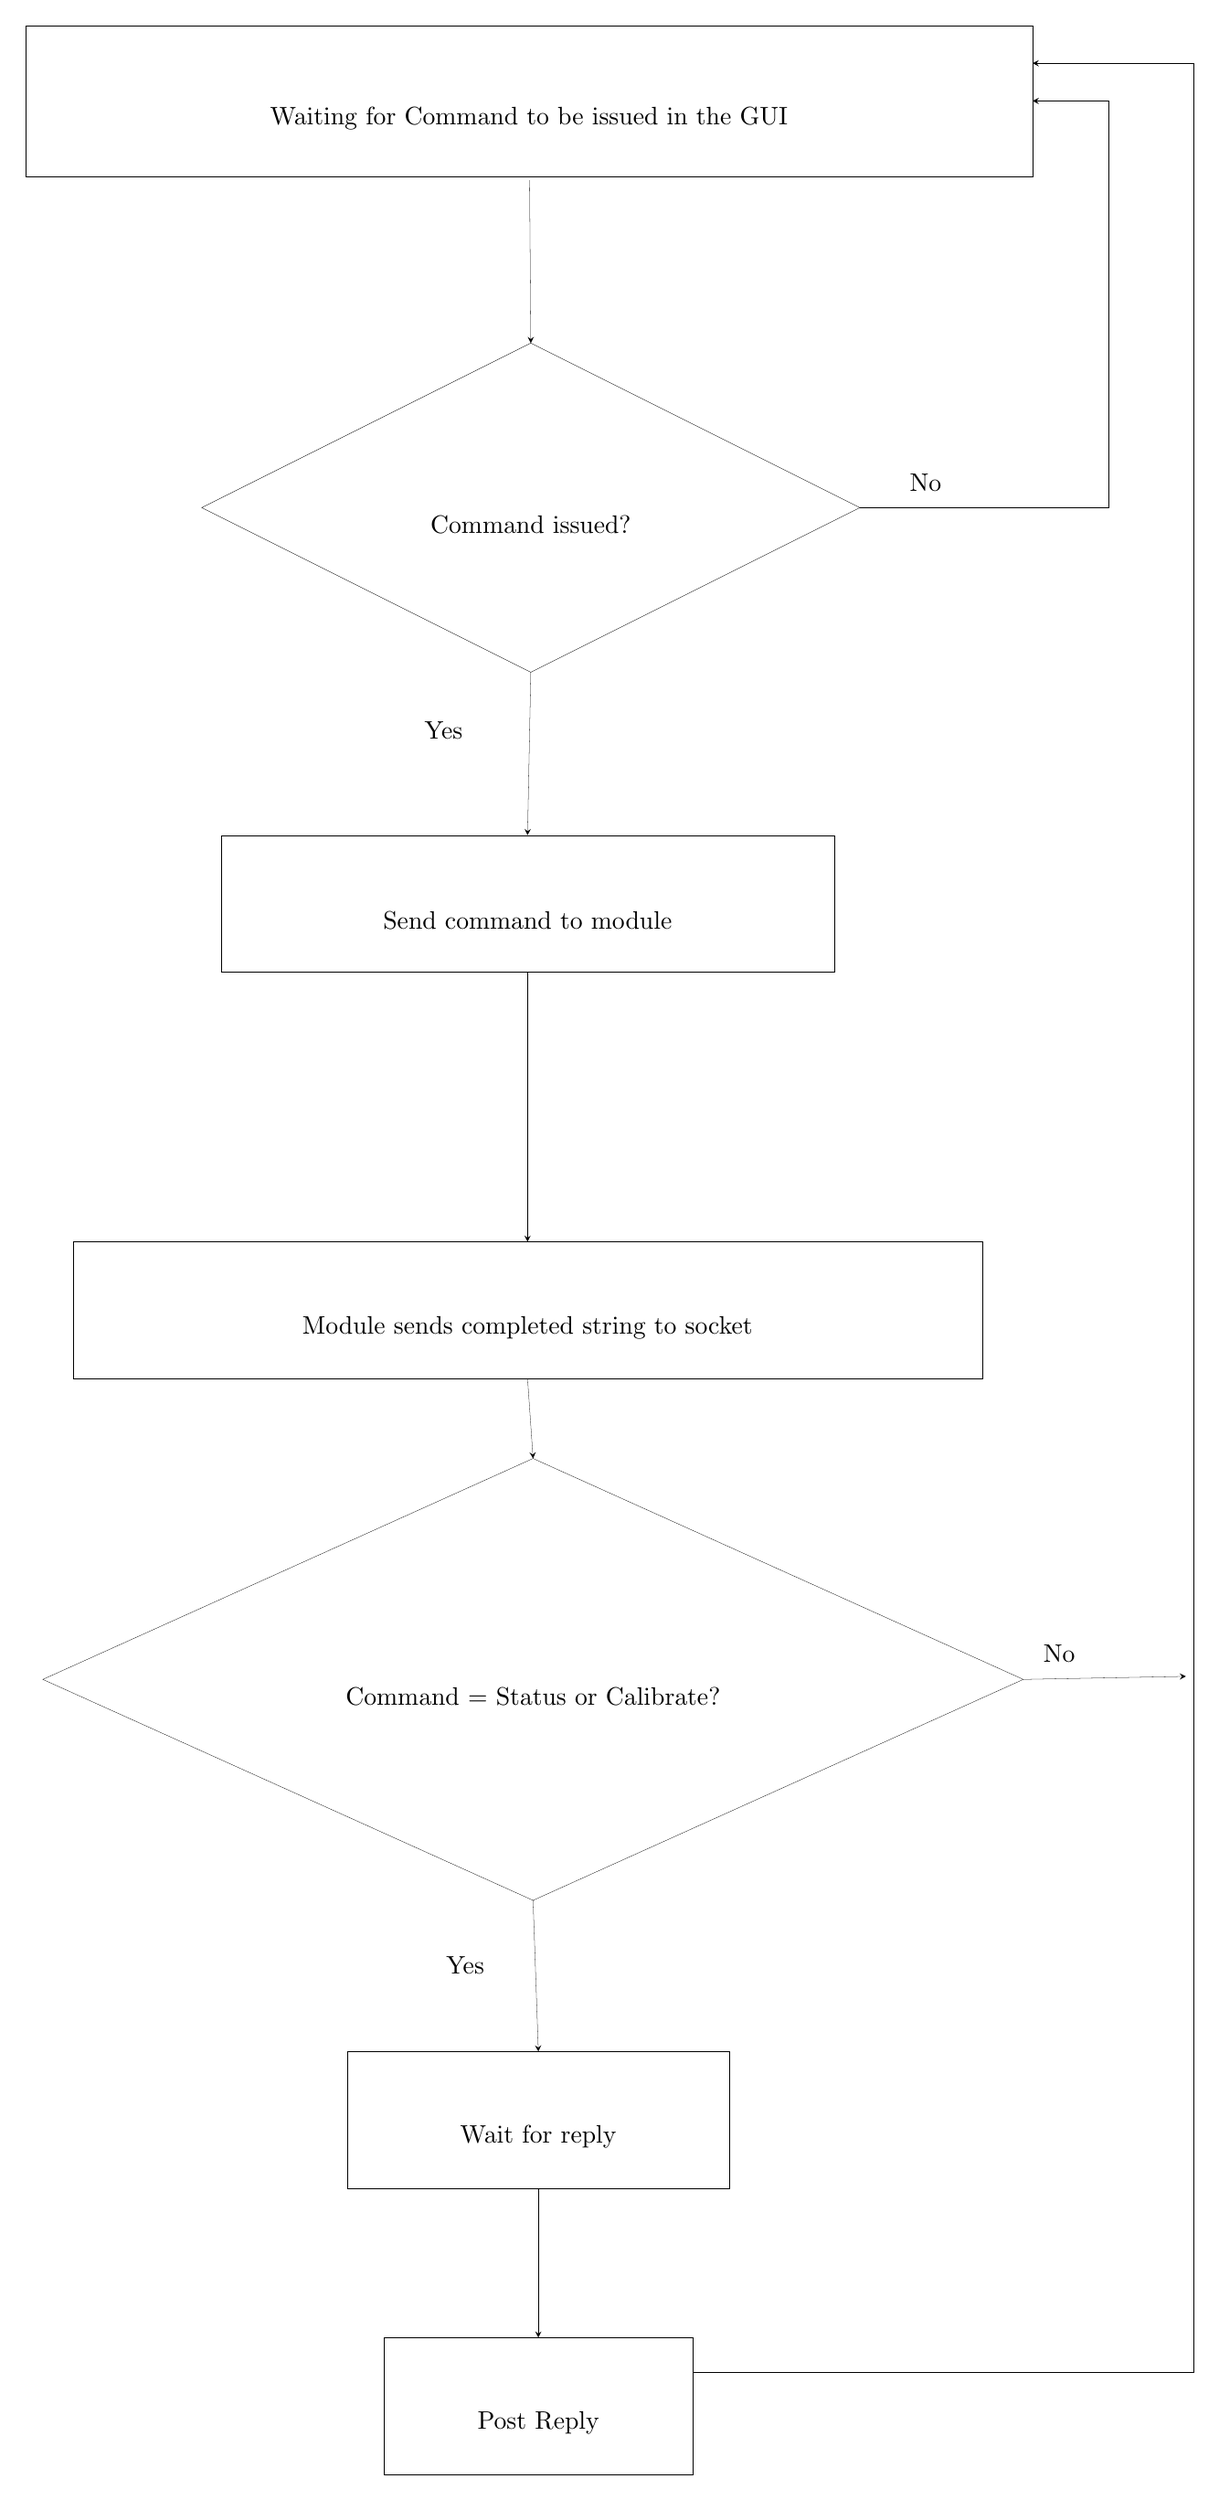
\begin{tikzpicture}
\pgftransformxscale{1.000000}
\pgftransformyscale{-1.000000}
\definecolor{dialinecolor}{rgb}{0.000000, 0.000000, 0.000000}
\pgfsetstrokecolor{dialinecolor}
\definecolor{dialinecolor}{rgb}{1.000000, 1.000000, 1.000000}
\pgfsetfillcolor{dialinecolor}
\definecolor{dialinecolor}{rgb}{1.000000, 1.000000, 1.000000}
\pgfsetfillcolor{dialinecolor}
\fill (5.726250\du,1.700000\du)--(5.726250\du,3.800000\du)--(19.723750\du,3.800000\du)--(19.723750\du,1.700000\du)--cycle;
\pgfsetlinewidth{0.100000\du}
\pgfsetdash{}{0pt}
\pgfsetdash{}{0pt}
\pgfsetmiterjoin
\definecolor{dialinecolor}{rgb}{0.000000, 0.000000, 0.000000}
\pgfsetstrokecolor{dialinecolor}
\draw (5.726250\du,1.700000\du)--(5.726250\du,3.800000\du)--(19.723750\du,3.800000\du)--(19.723750\du,1.700000\du)--cycle;
% setfont left to latex
\definecolor{dialinecolor}{rgb}{0.000000, 0.000000, 0.000000}
\pgfsetstrokecolor{dialinecolor}
\node at (12.725000\du,2.990000\du){Waiting for Command to be issued in the GUI};
\definecolor{dialinecolor}{rgb}{1.000000, 1.000000, 1.000000}
\pgfsetfillcolor{dialinecolor}
\fill (12.750000\du,6.113420\du)--(17.323160\du,8.400000\du)--(12.750000\du,10.686580\du)--(8.176840\du,8.400000\du)--cycle;
\pgfsetlinewidth{0.100000\du}
\pgfsetdash{}{0pt}
\pgfsetdash{}{0pt}
\pgfsetmiterjoin
\definecolor{dialinecolor}{rgb}{0.000000, 0.000000, 0.000000}
\pgfsetstrokecolor{dialinecolor}
\draw (12.750000\du,6.113420\du)--(17.323160\du,8.400000\du)--(12.750000\du,10.686580\du)--(8.176840\du,8.400000\du)--cycle;
% setfont left to latex
\definecolor{dialinecolor}{rgb}{0.000000, 0.000000, 0.000000}
\pgfsetstrokecolor{dialinecolor}
\node at (12.750000\du,8.640000\du){Command issued?};
\pgfsetlinewidth{0.100000\du}
\pgfsetdash{}{0pt}
\pgfsetdash{}{0pt}
\pgfsetmiterjoin
\pgfsetbuttcap
{
\definecolor{dialinecolor}{rgb}{0.000000, 0.000000, 0.000000}
\pgfsetfillcolor{dialinecolor}
% was here!!!
\pgfsetarrowsend{stealth}
{\pgfsetcornersarced{\pgfpoint{0.000000\du}{0.000000\du}}\definecolor{dialinecolor}{rgb}{0.000000, 0.000000, 0.000000}
\pgfsetstrokecolor{dialinecolor}
\draw (17.323200\du,8.400000\du)--(20.773800\du,8.400000\du)--(20.773800\du,2.750000\du)--(19.723800\du,2.750000\du);
}}
% setfont left to latex
\definecolor{dialinecolor}{rgb}{0.000000, 0.000000, 0.000000}
\pgfsetstrokecolor{dialinecolor}
\node[anchor=west] at (17.900000\du,8.050000\du){No};
\pgfsetlinewidth{0.100000\du}
\pgfsetdash{}{0pt}
\pgfsetdash{}{0pt}
\pgfsetbuttcap
{
\definecolor{dialinecolor}{rgb}{0.000000, 0.000000, 0.000000}
\pgfsetfillcolor{dialinecolor}
% was here!!!
\pgfsetarrowsend{stealth}
\definecolor{dialinecolor}{rgb}{0.000000, 0.000000, 0.000000}
\pgfsetstrokecolor{dialinecolor}
\draw (12.733167\du,3.848695\du)--(12.750000\du,6.113420\du);
}
\definecolor{dialinecolor}{rgb}{1.000000, 1.000000, 1.000000}
\pgfsetfillcolor{dialinecolor}
\fill (8.446350\du,12.950000\du)--(8.446350\du,14.850000\du)--(16.963850\du,14.850000\du)--(16.963850\du,12.950000\du)--cycle;
\pgfsetlinewidth{0.100000\du}
\pgfsetdash{}{0pt}
\pgfsetdash{}{0pt}
\pgfsetmiterjoin
\definecolor{dialinecolor}{rgb}{0.000000, 0.000000, 0.000000}
\pgfsetstrokecolor{dialinecolor}
\draw (8.446350\du,12.950000\du)--(8.446350\du,14.850000\du)--(16.963850\du,14.850000\du)--(16.963850\du,12.950000\du)--cycle;
% setfont left to latex
\definecolor{dialinecolor}{rgb}{0.000000, 0.000000, 0.000000}
\pgfsetstrokecolor{dialinecolor}
\node at (12.705100\du,14.140000\du){Send command to module};
\definecolor{dialinecolor}{rgb}{1.000000, 1.000000, 1.000000}
\pgfsetfillcolor{dialinecolor}
\fill (12.781577\du,21.610400\du)--(19.594965\du,24.680018\du)--(12.781577\du,27.749635\du)--(5.968190\du,24.680018\du)--cycle;
\pgfsetlinewidth{0.100000\du}
\pgfsetdash{}{0pt}
\pgfsetdash{}{0pt}
\pgfsetmiterjoin
\definecolor{dialinecolor}{rgb}{0.000000, 0.000000, 0.000000}
\pgfsetstrokecolor{dialinecolor}
\draw (12.781577\du,21.610400\du)--(19.594965\du,24.680018\du)--(12.781577\du,27.749635\du)--(5.968190\du,24.680018\du)--cycle;
% setfont left to latex
\definecolor{dialinecolor}{rgb}{0.000000, 0.000000, 0.000000}
\pgfsetstrokecolor{dialinecolor}
\node at (12.781577\du,24.920018\du){Command = Status or Calibrate?};
\definecolor{dialinecolor}{rgb}{1.000000, 1.000000, 1.000000}
\pgfsetfillcolor{dialinecolor}
\fill (10.202600\du,29.850000\du)--(10.202600\du,31.750000\du)--(15.507600\du,31.750000\du)--(15.507600\du,29.850000\du)--cycle;
\pgfsetlinewidth{0.100000\du}
\pgfsetdash{}{0pt}
\pgfsetdash{}{0pt}
\pgfsetmiterjoin
\definecolor{dialinecolor}{rgb}{0.000000, 0.000000, 0.000000}
\pgfsetstrokecolor{dialinecolor}
\draw (10.202600\du,29.850000\du)--(10.202600\du,31.750000\du)--(15.507600\du,31.750000\du)--(15.507600\du,29.850000\du)--cycle;
% setfont left to latex
\definecolor{dialinecolor}{rgb}{0.000000, 0.000000, 0.000000}
\pgfsetstrokecolor{dialinecolor}
\node at (12.855100\du,31.040000\du){Wait for reply};
\pgfsetlinewidth{0.100000\du}
\pgfsetdash{}{0pt}
\pgfsetdash{}{0pt}
\pgfsetbuttcap
{
\definecolor{dialinecolor}{rgb}{0.000000, 0.000000, 0.000000}
\pgfsetfillcolor{dialinecolor}
% was here!!!
\pgfsetarrowsend{stealth}
\definecolor{dialinecolor}{rgb}{0.000000, 0.000000, 0.000000}
\pgfsetstrokecolor{dialinecolor}
\draw (12.750000\du,10.686600\du)--(12.705100\du,12.950000\du);
}
\pgfsetlinewidth{0.100000\du}
\pgfsetdash{}{0pt}
\pgfsetdash{}{0pt}
\pgfsetbuttcap
{
\definecolor{dialinecolor}{rgb}{0.000000, 0.000000, 0.000000}
\pgfsetfillcolor{dialinecolor}
% was here!!!
\pgfsetarrowsend{stealth}
\definecolor{dialinecolor}{rgb}{0.000000, 0.000000, 0.000000}
\pgfsetstrokecolor{dialinecolor}
\draw (12.705100\du,14.850000\du)--(12.705100\du,18.600000\du);
}
% setfont left to latex
\definecolor{dialinecolor}{rgb}{0.000000, 0.000000, 0.000000}
\pgfsetstrokecolor{dialinecolor}
\node[anchor=west] at (11.155100\du,11.500000\du){Yes};
\pgfsetlinewidth{0.100000\du}
\pgfsetdash{}{0pt}
\pgfsetdash{}{0pt}
\pgfsetbuttcap
{
\definecolor{dialinecolor}{rgb}{0.000000, 0.000000, 0.000000}
\pgfsetfillcolor{dialinecolor}
% was here!!!
\pgfsetarrowsend{stealth}
\definecolor{dialinecolor}{rgb}{0.000000, 0.000000, 0.000000}
\pgfsetstrokecolor{dialinecolor}
\draw (12.781600\du,27.749700\du)--(12.855100\du,29.850000\du);
}
\definecolor{dialinecolor}{rgb}{1.000000, 1.000000, 1.000000}
\pgfsetfillcolor{dialinecolor}
\fill (6.386350\du,18.600000\du)--(6.386350\du,20.500000\du)--(19.023850\du,20.500000\du)--(19.023850\du,18.600000\du)--cycle;
\pgfsetlinewidth{0.100000\du}
\pgfsetdash{}{0pt}
\pgfsetdash{}{0pt}
\pgfsetmiterjoin
\definecolor{dialinecolor}{rgb}{0.000000, 0.000000, 0.000000}
\pgfsetstrokecolor{dialinecolor}
\draw (6.386350\du,18.600000\du)--(6.386350\du,20.500000\du)--(19.023850\du,20.500000\du)--(19.023850\du,18.600000\du)--cycle;
% setfont left to latex
\definecolor{dialinecolor}{rgb}{0.000000, 0.000000, 0.000000}
\pgfsetstrokecolor{dialinecolor}
\node at (12.705100\du,19.790000\du){Module sends completed string to socket};
\pgfsetlinewidth{0.100000\du}
\pgfsetdash{}{0pt}
\pgfsetdash{}{0pt}
\pgfsetbuttcap
{
\definecolor{dialinecolor}{rgb}{0.000000, 0.000000, 0.000000}
\pgfsetfillcolor{dialinecolor}
% was here!!!
\pgfsetarrowsend{stealth}
\definecolor{dialinecolor}{rgb}{0.000000, 0.000000, 0.000000}
\pgfsetstrokecolor{dialinecolor}
\draw (12.705100\du,20.500000\du)--(12.781600\du,21.610400\du);
}
\definecolor{dialinecolor}{rgb}{1.000000, 1.000000, 1.000000}
\pgfsetfillcolor{dialinecolor}
\fill (10.711400\du,33.825000\du)--(10.711400\du,35.725000\du)--(14.998900\du,35.725000\du)--(14.998900\du,33.825000\du)--cycle;
\pgfsetlinewidth{0.100000\du}
\pgfsetdash{}{0pt}
\pgfsetdash{}{0pt}
\pgfsetmiterjoin
\definecolor{dialinecolor}{rgb}{0.000000, 0.000000, 0.000000}
\pgfsetstrokecolor{dialinecolor}
\draw (10.711400\du,33.825000\du)--(10.711400\du,35.725000\du)--(14.998900\du,35.725000\du)--(14.998900\du,33.825000\du)--cycle;
% setfont left to latex
\definecolor{dialinecolor}{rgb}{0.000000, 0.000000, 0.000000}
\pgfsetstrokecolor{dialinecolor}
\node at (12.855150\du,35.015000\du){Post Reply};
\pgfsetlinewidth{0.100000\du}
\pgfsetdash{}{0pt}
\pgfsetdash{}{0pt}
\pgfsetbuttcap
{
\definecolor{dialinecolor}{rgb}{0.000000, 0.000000, 0.000000}
\pgfsetfillcolor{dialinecolor}
% was here!!!
\pgfsetarrowsend{stealth}
\definecolor{dialinecolor}{rgb}{0.000000, 0.000000, 0.000000}
\pgfsetstrokecolor{dialinecolor}
\draw (12.855100\du,31.750000\du)--(12.855100\du,33.825000\du);
}
\pgfsetlinewidth{0.100000\du}
\pgfsetdash{}{0pt}
\pgfsetdash{}{0pt}
\pgfsetmiterjoin
\pgfsetbuttcap
{
\definecolor{dialinecolor}{rgb}{0.000000, 0.000000, 0.000000}
\pgfsetfillcolor{dialinecolor}
% was here!!!
\pgfsetarrowsend{stealth}
{\pgfsetcornersarced{\pgfpoint{0.000000\du}{0.000000\du}}\definecolor{dialinecolor}{rgb}{0.000000, 0.000000, 0.000000}
\pgfsetstrokecolor{dialinecolor}
\draw (14.998900\du,34.300000\du)--(21.955100\du,34.300000\du)--(21.955100\du,2.225000\du)--(19.723800\du,2.225000\du);
}}
\pgfsetlinewidth{0.100000\du}
\pgfsetdash{}{0pt}
\pgfsetdash{}{0pt}
\pgfsetbuttcap
{
\definecolor{dialinecolor}{rgb}{0.000000, 0.000000, 0.000000}
\pgfsetfillcolor{dialinecolor}
% was here!!!
\pgfsetarrowsend{stealth}
\definecolor{dialinecolor}{rgb}{0.000000, 0.000000, 0.000000}
\pgfsetstrokecolor{dialinecolor}
\draw (19.595000\du,24.680000\du)--(21.855100\du,24.637500\du);
}
% setfont left to latex
\definecolor{dialinecolor}{rgb}{0.000000, 0.000000, 0.000000}
\pgfsetstrokecolor{dialinecolor}
\node[anchor=west] at (19.755100\du,24.325000\du){No};
% setfont left to latex
\definecolor{dialinecolor}{rgb}{0.000000, 0.000000, 0.000000}
\pgfsetstrokecolor{dialinecolor}
\node[anchor=west] at (11.455100\du,28.650000\du){Yes};
\end{tikzpicture}
}
  \caption{Flödesschema över mjukvaran på PC}
\end{figure}

\subsection{Komponenter}
\begin{itemize}
\item En PC med ett JÄVLIGT BRA operativsystem och Python 3 installerat
\item En Blåtandsdongel till PC:n
\end{itemize}


\section{Huvudmodul}
Huvudmodulen kan ses som systemets "hjärna". Här sker alla beräkningar för att roboten ska kunna utföra sina uppgifter. Dessa uppgifter ska huvudmodulen hantera antingen via kommandon från en PC eller skötas helt autonomt. Detta är en kritisk modul då den kommer att utföra mycket uppgifter. Den behöver inte mycket hårdvara men den kommer vara mjukvarutung.
\subsection{Hårdvara}
Modulen ska förslagsvis bestå av en enkortsdator av modell Beagleboard. Den har en ARM Cortex-A8 processor som har en klockfrekvens på 1GHz. Denna behöver ett operativsystem för att kunna användas. Den enda hårdvaran som behövs för att kunna använda BB är ett minneskort för operativsystem och en bluetooth-dongel för kommunikationen med PC:n. För kommunikationen med styrenhet och sensorenheten behöver vi 
\subsection{Mjukvara}
% Graphic for TeX using PGF
% Title: /home/martin/Downloads/trådar.dia
% Creator: Dia v0.97.2
% CreationDate: Mon Oct  6 14:56:04 2014
% For: martin
% \usepackage{tikz}
% The following commands are not supported in PSTricks at present
% We define them conditionally, so when they are implemented,
% this pgf file will use them.
\ifx\du\undefined
  \newlength{\du}
\fi
\setlength{\du}{15\unitlength}
\begin{tikzpicture}
\pgftransformxscale{1.000000}
\pgftransformyscale{-1.000000}
\definecolor{dialinecolor}{rgb}{0.000000, 0.000000, 0.000000}
\pgfsetstrokecolor{dialinecolor}
\definecolor{dialinecolor}{rgb}{1.000000, 1.000000, 1.000000}
\pgfsetfillcolor{dialinecolor}
\pgfsetlinewidth{0.100000\du}
\pgfsetdash{}{0pt}
\definecolor{dialinecolor}{rgb}{1.000000, 1.000000, 1.000000}
\pgfsetfillcolor{dialinecolor}
\fill (83.362742\du,-37.782161\du)--(83.362742\du,-36.382161\du)--(89.792742\du,-36.382161\du)--(89.792742\du,-37.782161\du)--cycle;
\definecolor{dialinecolor}{rgb}{0.000000, 0.000000, 0.000000}
\pgfsetstrokecolor{dialinecolor}
\draw (83.362742\du,-37.782161\du)--(83.362742\du,-36.382161\du)--(89.792742\du,-36.382161\du)--(89.792742\du,-37.782161\du)--cycle;
% setfont left to latex
\definecolor{dialinecolor}{rgb}{0.000000, 0.000000, 0.000000}
\pgfsetstrokecolor{dialinecolor}
\node at (86.577742\du,-36.832161\du){HUVUD-TRÅD};
\pgfsetlinewidth{0.100000\du}
\pgfsetdash{}{0pt}
\definecolor{dialinecolor}{rgb}{1.000000, 1.000000, 1.000000}
\pgfsetfillcolor{dialinecolor}
\fill (70.982742\du,-37.669161\du)--(70.982742\du,-36.269161\du)--(77.805242\du,-36.269161\du)--(77.805242\du,-37.669161\du)--cycle;
\definecolor{dialinecolor}{rgb}{0.000000, 0.000000, 0.000000}
\pgfsetstrokecolor{dialinecolor}
\draw (70.982742\du,-37.669161\du)--(70.982742\du,-36.269161\du)--(77.805242\du,-36.269161\du)--(77.805242\du,-37.669161\du)--cycle;
% setfont left to latex
\definecolor{dialinecolor}{rgb}{0.000000, 0.000000, 0.000000}
\pgfsetstrokecolor{dialinecolor}
\node at (74.393992\du,-36.719161\du){SENSOR-TRÅD};
\pgfsetlinewidth{0.100000\du}
\pgfsetdash{}{0pt}
\definecolor{dialinecolor}{rgb}{1.000000, 1.000000, 1.000000}
\pgfsetfillcolor{dialinecolor}
\fill (76.282742\du,-33.369161\du)--(76.282742\du,-31.969161\du)--(82.932742\du,-31.969161\du)--(82.932742\du,-33.369161\du)--cycle;
\definecolor{dialinecolor}{rgb}{0.000000, 0.000000, 0.000000}
\pgfsetstrokecolor{dialinecolor}
\draw (76.282742\du,-33.369161\du)--(76.282742\du,-31.969161\du)--(82.932742\du,-31.969161\du)--(82.932742\du,-33.369161\du)--cycle;
% setfont left to latex
\definecolor{dialinecolor}{rgb}{0.000000, 0.000000, 0.000000}
\pgfsetstrokecolor{dialinecolor}
\node at (79.607742\du,-32.419161\du){sensorvärden};
\definecolor{dialinecolor}{rgb}{1.000000, 1.000000, 1.000000}
\pgfsetfillcolor{dialinecolor}
\fill (76.282742\du,-31.969161\du)--(76.282742\du,-31.569161\du)--(82.932742\du,-31.569161\du)--(82.932742\du,-31.969161\du)--cycle;
\definecolor{dialinecolor}{rgb}{0.000000, 0.000000, 0.000000}
\pgfsetstrokecolor{dialinecolor}
\draw (76.282742\du,-31.969161\du)--(76.282742\du,-31.569161\du)--(82.932742\du,-31.569161\du)--(82.932742\du,-31.969161\du)--cycle;
\definecolor{dialinecolor}{rgb}{1.000000, 1.000000, 1.000000}
\pgfsetfillcolor{dialinecolor}
\fill (76.282742\du,-31.569161\du)--(76.282742\du,-31.169161\du)--(82.932742\du,-31.169161\du)--(82.932742\du,-31.569161\du)--cycle;
\definecolor{dialinecolor}{rgb}{0.000000, 0.000000, 0.000000}
\pgfsetstrokecolor{dialinecolor}
\draw (76.282742\du,-31.569161\du)--(76.282742\du,-31.169161\du)--(82.932742\du,-31.169161\du)--(82.932742\du,-31.569161\du)--cycle;
\pgfsetlinewidth{0.100000\du}
\pgfsetdash{}{0pt}
\definecolor{dialinecolor}{rgb}{1.000000, 1.000000, 1.000000}
\pgfsetfillcolor{dialinecolor}
\fill (88.732742\du,-33.369161\du)--(88.732742\du,-31.969161\du)--(94.760242\du,-31.969161\du)--(94.760242\du,-33.369161\du)--cycle;
\definecolor{dialinecolor}{rgb}{0.000000, 0.000000, 0.000000}
\pgfsetstrokecolor{dialinecolor}
\draw (88.732742\du,-33.369161\du)--(88.732742\du,-31.969161\du)--(94.760242\du,-31.969161\du)--(94.760242\du,-33.369161\du)--cycle;
% setfont left to latex
\definecolor{dialinecolor}{rgb}{0.000000, 0.000000, 0.000000}
\pgfsetstrokecolor{dialinecolor}
\node at (91.746492\du,-32.419161\du){instruktioner};
\definecolor{dialinecolor}{rgb}{1.000000, 1.000000, 1.000000}
\pgfsetfillcolor{dialinecolor}
\fill (88.732742\du,-31.969161\du)--(88.732742\du,-31.569161\du)--(94.760242\du,-31.569161\du)--(94.760242\du,-31.969161\du)--cycle;
\definecolor{dialinecolor}{rgb}{0.000000, 0.000000, 0.000000}
\pgfsetstrokecolor{dialinecolor}
\draw (88.732742\du,-31.969161\du)--(88.732742\du,-31.569161\du)--(94.760242\du,-31.569161\du)--(94.760242\du,-31.969161\du)--cycle;
\definecolor{dialinecolor}{rgb}{1.000000, 1.000000, 1.000000}
\pgfsetfillcolor{dialinecolor}
\fill (88.732742\du,-31.569161\du)--(88.732742\du,-31.169161\du)--(94.760242\du,-31.169161\du)--(94.760242\du,-31.569161\du)--cycle;
\definecolor{dialinecolor}{rgb}{0.000000, 0.000000, 0.000000}
\pgfsetstrokecolor{dialinecolor}
\draw (88.732742\du,-31.569161\du)--(88.732742\du,-31.169161\du)--(94.760242\du,-31.169161\du)--(94.760242\du,-31.569161\du)--cycle;
\pgfsetlinewidth{0.100000\du}
\pgfsetdash{}{0pt}
\definecolor{dialinecolor}{rgb}{1.000000, 1.000000, 1.000000}
\pgfsetfillcolor{dialinecolor}
\fill (97.282742\du,-37.657161\du)--(97.282742\du,-36.257161\du)--(101.635242\du,-36.257161\du)--(101.635242\du,-37.657161\du)--cycle;
\definecolor{dialinecolor}{rgb}{0.000000, 0.000000, 0.000000}
\pgfsetstrokecolor{dialinecolor}
\draw (97.282742\du,-37.657161\du)--(97.282742\du,-36.257161\du)--(101.635242\du,-36.257161\du)--(101.635242\du,-37.657161\du)--cycle;
% setfont left to latex
\definecolor{dialinecolor}{rgb}{0.000000, 0.000000, 0.000000}
\pgfsetstrokecolor{dialinecolor}
\node at (99.458992\du,-36.707161\du){PC-TRÅD};
\pgfsetlinewidth{0.100000\du}
\pgfsetdash{}{0pt}
\pgfsetdash{}{0pt}
\pgfsetbuttcap
{
\definecolor{dialinecolor}{rgb}{0.000000, 0.000000, 0.000000}
\pgfsetfillcolor{dialinecolor}
% was here!!!
\pgfsetarrowsstart{stealth}
\pgfsetarrowsend{stealth}
\definecolor{dialinecolor}{rgb}{0.000000, 0.000000, 0.000000}
\pgfsetstrokecolor{dialinecolor}
\draw (81.072842\du,-33.469161\du)--(85.291242\du,-36.382161\du);
}
\pgfsetlinewidth{0.100000\du}
\pgfsetdash{}{0pt}
\pgfsetdash{}{0pt}
\pgfsetbuttcap
{
\definecolor{dialinecolor}{rgb}{0.000000, 0.000000, 0.000000}
\pgfsetfillcolor{dialinecolor}
% was here!!!
\pgfsetarrowsend{stealth}
\definecolor{dialinecolor}{rgb}{0.000000, 0.000000, 0.000000}
\pgfsetstrokecolor{dialinecolor}
\draw (75.225188\du,-36.219869\du)--(78.331671\du,-33.419491\du);
}
\pgfsetlinewidth{0.100000\du}
\pgfsetdash{}{0pt}
\pgfsetdash{}{0pt}
\pgfsetmiterjoin
\pgfsetbuttcap
{
\definecolor{dialinecolor}{rgb}{0.000000, 0.000000, 0.000000}
\pgfsetfillcolor{dialinecolor}
% was here!!!
\pgfsetarrowsend{stealth}
{\pgfsetcornersarced{\pgfpoint{0.000000\du}{0.000000\du}}\definecolor{dialinecolor}{rgb}{0.000000, 0.000000, 0.000000}
\pgfsetstrokecolor{dialinecolor}
\draw (79.607742\du,-31.169161\du)--(79.607742\du,-27.644161\du)--(99.458992\du,-27.644161\du)--(99.458992\du,-36.257161\du);
}}
\pgfsetlinewidth{0.100000\du}
\pgfsetdash{}{0pt}
\pgfsetdash{}{0pt}
\pgfsetbuttcap
{
\definecolor{dialinecolor}{rgb}{0.000000, 0.000000, 0.000000}
\pgfsetfillcolor{dialinecolor}
% was here!!!
\pgfsetarrowsstart{to}
\pgfsetarrowsend{stealth}
\definecolor{dialinecolor}{rgb}{0.000000, 0.000000, 0.000000}
\pgfsetstrokecolor{dialinecolor}
\draw (93.732742\du,-33.444161\du)--(99.458992\du,-36.257161\du);
}
\pgfsetlinewidth{0.100000\du}
\pgfsetdash{}{0pt}
\pgfsetdash{}{0pt}
\pgfsetbuttcap
{
\definecolor{dialinecolor}{rgb}{0.000000, 0.000000, 0.000000}
\pgfsetfillcolor{dialinecolor}
% was here!!!
\pgfsetarrowsstart{stealth}
\definecolor{dialinecolor}{rgb}{0.000000, 0.000000, 0.000000}
\pgfsetstrokecolor{dialinecolor}
\draw (87.782742\du,-36.282161\du)--(91.746492\du,-33.369161\du);
}
\pgfsetlinewidth{0.100000\du}
\pgfsetdash{}{0pt}
\pgfsetdash{}{0pt}
\pgfsetmiterjoin
\pgfsetbuttcap
{
\definecolor{dialinecolor}{rgb}{0.000000, 0.000000, 0.000000}
\pgfsetfillcolor{dialinecolor}
% was here!!!
\pgfsetarrowsstart{stealth}
{\pgfsetcornersarced{\pgfpoint{0.000000\du}{0.000000\du}}\definecolor{dialinecolor}{rgb}{0.000000, 0.000000, 0.000000}
\pgfsetstrokecolor{dialinecolor}
\draw (74.393992\du,-37.669161\du)--(74.393992\du,-42.382161\du)--(92.582742\du,-42.382161\du)--(92.582742\du,-33.432161\du);
}}
\end{tikzpicture}

\subsubsection{Autonomt läge}
När roboten är satt i autonomt läge kommer all styrning skötas av en algoritm i huvudmodulen, med undantag för upphämtning av paket där användaren styr armen. Detta är en väldigt kritisk del då detta är denna algoritm som avgör robotens beteende och som sedan kommer leda till att den kan fullfölja sina uppgifter. Troligtvis kommer en stor del av tiden läggas på att felsöka och optimera algoritmen.
För att roboten ska kunna färdas framåt smidigt så kommer den behöva någon slags reglering. Förslagsvis ska en PD reglering implementeras som arbetar tidsdiskret. Detta gör att man måste sampla data från linjesensorerna med att visst intervall. Detta intervall är ej bestämt än.



\begin{figure}[h]
\center
\includegraphics[scale=0.2]{Styrlogik.png}
\caption{Flödesschema för huvudmodulens styralgoritm.} \label{systemskiss:autonomtschema}
\end{figure}

Figur \ref{systemskiss:autonomtschema} är en visualisering av hur det autonoma läget kommer att styras. Med hjälp av två stycken flaggor, Upplockning och Avplockning, kan systemet avgöra om den ska plocka upp eller lämna av ett paket eller bara fortsätta köra framåt längs banan. När Upplockning är satt till "Ja" väntar systemet på att användaren ska styra armen och sedan skicka ett "färdigt-kommando".

\subsubsection{Manuellt läge}
När roboten är satt i manuellt läge väntar huvudmodulen på kommandon från användaren och utför sedan dessa. 


\subsection{Kommunikation}
\subsubsection{Huvudmodul-PC}
\subsubsection{Huvudmodul-Styrenhet}
\subsubsection{Huvudmodul-Sensorenhet}
\subsection{Reglering}
För att undvika att roboten hackar sig fram och får en smidig rörelse så ska motorns styrsignaler regleras med en tidsdiskret PD-regulator. En PID regulator är onödig då vi inte har något stående fel i teorin. Om roboten är mitt på linjen och står rakt så kommer felet vara noll. I praktiken kommer det inte vara så då roboten troligtvis inte kommer stå rakt på linejn och motorerna kommer säkert åka i olika hastigheter. Dock så blir en PD-regulator tillräckligt bra. En annan anledning till att inte ha med I-delen är att det är svårt att implementera det bra i ett tidsdiskret system. e[n] Är felet vid sampling n. 
\begin{itemize}
\item e[n] Är felet vid sampling n
\item e[n-1] Är felet vid sampling n-1
\item u[n] är styrsignalen till motorerna
\item K\_P är en konstant för den proportionella delen av regleringen
\item K\_D är en konstant för den deriverande delen av regleringen
\item Delta T är tiden mellan sampling n och n-1
 
\end{itemize}
 $$ u[n] = K_P*e[n] + K_D\frac{e[n]-e[n-1]}{\Delta T}$$
 Roboten är begränsade av hårdvaran hur ofta den kan läsa av data från reflexsensorna. Enligt handledaren är en uppdatering på 25 Hertz en rimlig nivå. Så delta T kommer vara 40ms
\subsection{hårdvara som behövs}
\begin{itemize}
\item Beagleboard-xm (finns i vanheden)
\item BT-dongle Belkin f8t016(vi har en)
\item Nivåomvandlare Ti TXB0108 ("http://www.electrokit.com/nivaomvandlare-8-kanaler.50717")
\item Minneskort (Om det inte finns i vanheden så beställ från elfa )
\item Wifi dongel för utveckling på den (vi har en)
\end{itemize}


%\documentclass[a4paper,11pt]{article}
%\usepackage[a4paper]{}
%\usepackage[utf8]{inputenc}
%\usepackage{listings}
%\usepackage{graphicx}
%\begin{document}

\section{Sensorenhet}
Sensorenheten har till uppgift att läsa in data från robotens sensorer, tolka den och vidarebefodra den till huvudmodulen. En reflexsensormodul används för att roboten skall kunna hålla sig på banan. För att kunna detektera paket kommer roboten ha en avståndssensor på vardera sida. \\

\begin{figure}[h]
\center
% Graphic for TeX using PGF
% Title: /home/kebabdjuret/Documents/skola/tsea29/gloria/dokumentation/designspecifikation/sensorenhet-blockschema.dia
% Creator: Dia v0.97.2
% CreationDate: Thu Oct  9 14:42:10 2014
% For: kebabdjuret
% \usepackage{tikz}
% The following commands are not supported in PSTricks at present
% We define them conditionally, so when they are implemented,
% this pgf file will use them.
\ifx\du\undefined
  \newlength{\du}
\fi
\setlength{\du}{15\unitlength}
\begin{tikzpicture}
\pgftransformxscale{1.000000}
\pgftransformyscale{-1.000000}
\definecolor{dialinecolor}{rgb}{0.000000, 0.000000, 0.000000}
\pgfsetstrokecolor{dialinecolor}
\definecolor{dialinecolor}{rgb}{1.000000, 1.000000, 1.000000}
\pgfsetfillcolor{dialinecolor}
\pgfsetlinewidth{0.100000\du}
\pgfsetdash{}{0pt}
\pgfsetdash{}{0pt}
\pgfsetmiterjoin
\definecolor{dialinecolor}{rgb}{1.000000, 1.000000, 1.000000}
\pgfsetfillcolor{dialinecolor}
\fill (15.427300\du,9.486540\du)--(15.427300\du,17.645911\du)--(20.127300\du,17.645911\du)--(20.127300\du,9.486540\du)--cycle;
\definecolor{dialinecolor}{rgb}{0.000000, 0.000000, 0.000000}
\pgfsetstrokecolor{dialinecolor}
\draw (15.427300\du,9.486540\du)--(15.427300\du,17.645911\du)--(20.127300\du,17.645911\du)--(20.127300\du,9.486540\du)--cycle;
\pgfsetlinewidth{0.100000\du}
\pgfsetdash{}{0pt}
\pgfsetdash{}{0pt}
\pgfsetmiterjoin
\definecolor{dialinecolor}{rgb}{1.000000, 1.000000, 1.000000}
\pgfsetfillcolor{dialinecolor}
\fill (25.040900\du,10.114600\du)--(25.040900\du,12.022980\du)--(33.816769\du,12.022980\du)--(33.816769\du,10.114600\du)--cycle;
\definecolor{dialinecolor}{rgb}{0.000000, 0.000000, 0.000000}
\pgfsetstrokecolor{dialinecolor}
\draw (25.040900\du,10.114600\du)--(25.040900\du,12.022980\du)--(33.816769\du,12.022980\du)--(33.816769\du,10.114600\du)--cycle;
\pgfsetlinewidth{0.100000\du}
\pgfsetdash{}{0pt}
\pgfsetdash{}{0pt}
\pgfsetmiterjoin
\definecolor{dialinecolor}{rgb}{1.000000, 1.000000, 1.000000}
\pgfsetfillcolor{dialinecolor}
\fill (25.039100\du,12.551500\du)--(25.039100\du,14.459880\du)--(33.816769\du,14.459880\du)--(33.816769\du,12.551500\du)--cycle;
\definecolor{dialinecolor}{rgb}{0.000000, 0.000000, 0.000000}
\pgfsetstrokecolor{dialinecolor}
\draw (25.039100\du,12.551500\du)--(25.039100\du,14.459880\du)--(33.816769\du,14.459880\du)--(33.816769\du,12.551500\du)--cycle;
\pgfsetlinewidth{0.100000\du}
\pgfsetdash{}{0pt}
\pgfsetdash{}{0pt}
\pgfsetbuttcap
{
\definecolor{dialinecolor}{rgb}{0.000000, 0.000000, 0.000000}
\pgfsetfillcolor{dialinecolor}
% was here!!!
\pgfsetarrowsend{to}
\definecolor{dialinecolor}{rgb}{0.000000, 0.000000, 0.000000}
\pgfsetstrokecolor{dialinecolor}
\draw (25.040900\du,11.068790\du)--(20.106300\du,11.102900\du);
}
\pgfsetlinewidth{0.100000\du}
\pgfsetdash{}{0pt}
\pgfsetdash{}{0pt}
\pgfsetbuttcap
{
\definecolor{dialinecolor}{rgb}{0.000000, 0.000000, 0.000000}
\pgfsetfillcolor{dialinecolor}
% was here!!!
\pgfsetarrowsend{to}
\definecolor{dialinecolor}{rgb}{0.000000, 0.000000, 0.000000}
\pgfsetstrokecolor{dialinecolor}
\draw (25.039100\du,13.505690\du)--(20.077600\du,13.540100\du);
}
% setfont left to latex
\definecolor{dialinecolor}{rgb}{0.000000, 0.000000, 0.000000}
\pgfsetstrokecolor{dialinecolor}
\node[anchor=west] at (17.189200\du,13.801900\du){AVR};
\pgfsetlinewidth{0.100000\du}
\pgfsetdash{}{0pt}
\pgfsetdash{}{0pt}
\pgfsetbuttcap
{
\definecolor{dialinecolor}{rgb}{0.000000, 0.000000, 0.000000}
\pgfsetfillcolor{dialinecolor}
% was here!!!
\pgfsetarrowsstart{to}
\pgfsetarrowsend{to}
\definecolor{dialinecolor}{rgb}{0.000000, 0.000000, 0.000000}
\pgfsetstrokecolor{dialinecolor}
\draw (11.216500\du,13.588400\du)--(15.427300\du,13.566200\du);
}
\pgfsetlinewidth{0.100000\du}
\pgfsetdash{}{0pt}
\pgfsetdash{}{0pt}
\pgfsetmiterjoin
\definecolor{dialinecolor}{rgb}{1.000000, 1.000000, 1.000000}
\pgfsetfillcolor{dialinecolor}
\fill (6.691550\du,13.088400\du)--(6.691550\du,14.088391\du)--(11.216510\du,14.088391\du)--(11.216510\du,13.088400\du)--cycle;
\definecolor{dialinecolor}{rgb}{0.000000, 0.000000, 0.000000}
\pgfsetstrokecolor{dialinecolor}
\draw (6.691550\du,13.088400\du)--(6.691550\du,14.088391\du)--(11.216510\du,14.088391\du)--(11.216510\du,13.088400\du)--cycle;
% setfont left to latex
\definecolor{dialinecolor}{rgb}{0.000000, 0.000000, 0.000000}
\pgfsetstrokecolor{dialinecolor}
\node[anchor=west] at (7.016550\du,13.788400\du){Huvudenhet};
% setfont left to latex
\definecolor{dialinecolor}{rgb}{0.000000, 0.000000, 0.000000}
\pgfsetstrokecolor{dialinecolor}
\node[anchor=west] at (12.814700\du,13.430700\du){SPI};
\pgfsetlinewidth{0.100000\du}
\pgfsetdash{}{0pt}
\pgfsetdash{}{0pt}
\pgfsetbuttcap
{
\definecolor{dialinecolor}{rgb}{0.000000, 0.000000, 0.000000}
\pgfsetfillcolor{dialinecolor}
% was here!!!
\pgfsetarrowsend{to}
\definecolor{dialinecolor}{rgb}{0.000000, 0.000000, 0.000000}
\pgfsetstrokecolor{dialinecolor}
\draw (17.799700\du,20.290500\du)--(17.777300\du,17.645900\du);
}
% setfont left to latex
\definecolor{dialinecolor}{rgb}{0.000000, 0.000000, 0.000000}
\pgfsetstrokecolor{dialinecolor}
\node[anchor=west] at (17.099700\du,20.965500\du){JTAG};
% setfont left to latex
\definecolor{dialinecolor}{rgb}{0.000000, 0.000000, 0.000000}
\pgfsetstrokecolor{dialinecolor}
\node[anchor=west] at (21.691337\du,10.613944\du){Analog};
% setfont left to latex
\definecolor{dialinecolor}{rgb}{0.000000, 0.000000, 0.000000}
\pgfsetstrokecolor{dialinecolor}
\node[anchor=west] at (21.727000\du,13.001822\du){Analog};
% setfont left to latex
\definecolor{dialinecolor}{rgb}{0.000000, 0.000000, 0.000000}
\pgfsetstrokecolor{dialinecolor}
\node[anchor=west] at (29.428835\du,11.068790\du){};
% setfont left to latex
\definecolor{dialinecolor}{rgb}{0.000000, 0.000000, 0.000000}
\pgfsetstrokecolor{dialinecolor}
\node[anchor=west] at (25.581850\du,11.132679\du){Vänster avståndssensor};
% setfont left to latex
\definecolor{dialinecolor}{rgb}{0.000000, 0.000000, 0.000000}
\pgfsetstrokecolor{dialinecolor}
\node[anchor=west] at (25.841217\du,13.629092\du){Höger avståndssensor};
\pgfsetlinewidth{0.100000\du}
\pgfsetdash{}{0pt}
\pgfsetdash{}{0pt}
\pgfsetmiterjoin
\definecolor{dialinecolor}{rgb}{1.000000, 1.000000, 1.000000}
\pgfsetfillcolor{dialinecolor}
\fill (24.998273\du,15.152876\du)--(24.998273\du,17.065712\du)--(33.849190\du,17.065712\du)--(33.849190\du,15.152876\du)--cycle;
\definecolor{dialinecolor}{rgb}{0.000000, 0.000000, 0.000000}
\pgfsetstrokecolor{dialinecolor}
\draw (24.998273\du,15.152876\du)--(24.998273\du,17.065712\du)--(33.849190\du,17.065712\du)--(33.849190\du,15.152876\du)--cycle;
% setfont left to latex
\definecolor{dialinecolor}{rgb}{0.000000, 0.000000, 0.000000}
\pgfsetstrokecolor{dialinecolor}
\node[anchor=west] at (29.423732\du,16.109294\du){  };
\pgfsetlinewidth{0.100000\du}
\pgfsetdash{}{0pt}
\pgfsetdash{}{0pt}
\pgfsetbuttcap
{
\definecolor{dialinecolor}{rgb}{0.000000, 0.000000, 0.000000}
\pgfsetfillcolor{dialinecolor}
% was here!!!
\pgfsetarrowsend{to}
\definecolor{dialinecolor}{rgb}{0.000000, 0.000000, 0.000000}
\pgfsetstrokecolor{dialinecolor}
\draw (24.998273\du,16.109294\du)--(20.135132\du,16.125505\du);
}
% setfont left to latex
\definecolor{dialinecolor}{rgb}{0.000000, 0.000000, 0.000000}
\pgfsetstrokecolor{dialinecolor}
\node[anchor=west] at (21.629737\du,15.530656\du){Analog};
% setfont left to latex
\definecolor{dialinecolor}{rgb}{0.000000, 0.000000, 0.000000}
\pgfsetstrokecolor{dialinecolor}
\node[anchor=west] at (27.429844\du,16.255188\du){Reflexsensor};
\end{tikzpicture}

\caption{Blockschema över sensorenheten}
\end{figure}

\subsection{Reflexsensormodul}
Reflexsensormodulen består av 11 reflexsensorer. En reflexsensor består av en lysdiod och en fototransistor. Fototransistorn har ett analogt utvärde mellan 0 och 5V beroende på hur mycket ljus som fångas upp. Genom att sätta enable för en lysdiod till 1 och sedan läsa av den tillhörande fototransistorn kan vi avgöra om underlaget är ljust eller mörkt. Fototransistorn läses av med en AD-omvandling på AVRen. Detta görs för varje reflexsensor och på så sätt kan vi detektera tejpens position under sensorn eftersom tejpen banan består av får förutsättas ha en annan färg än golvet. Eftersom AVRen har ett begränsat antal pinnar med AD-omvandling, muxar vi fototransistorernas utgångar till en enda pinne på AVRen. Då vi inte vill ha mer än en lysdiod igång samtidigt kommer vi använda ytterligare en mux för att styra en enablesignal till den lysdiod vi vill använda, övriga kommer vara avslagna.

\subsubsection{Kalibrering}
Beroende på vilket underlag roboten arbetar på kommer värdena för golv och tejp att variera. Vi behöver därför kunna kalibrera sensorn för att sätta standardvärden. Detta kommer ske på ett sådant sätt att vi först låter roboten titta på bara golvet och sedan en bit tejp. Vi sparar de värden vi får under dessa testfall och använder dem som referens när vi ska detektera golv eller tejp.

\subsection{Avståndssensor}
För att kunna detektera paket kommer roboten ha en avståndssensor på höger respektive vänster sida. Dessa kommer vara av typen GP2D120 och använder IR för att generera en analog signal. Denna signal läses av med en AD-omvandling på AVRen. Då sensorns utsignal är olinjär kommer vi under utveckligsfasen ta fram en tabell med närmevärden för olika distanser. Utsignalen jämförs med denna tabell för att estimera det uppmätta avståndet till ett föremål.

\subsection{Hårdvara}
Till sensorenheten krävs följande hårdvara.
\begin{itemize}
\item{En AVR av typ Atmega16}
\item{En Reflexsensormodul}
\item{Två muxar av typ MC14067B}
\item{Två avståndssensorer av typ GP2D120}
\item{En JTAG Ice 3}
\end{itemize}

\subsection{Mjukvara}
Sensorenheten kör kontinuerligt en loop där den läser och lagrar data från sensorerna. Då huvudenheten skickar en instruktion till sensorenheten körs en avbrottsrutin där instruktionen tolkas och utförs. Antingen kalibreras sensorerna eller så returnerar sensorenheten data för den adresserade sensorn.

%Figur \ref{systemskiss:sensorschema} visar flödesschema över mjukvaran i sensormodulen.

%\begin{figure}[h]
%\center
%\includegraphics[scale=0.4]{sensorflow}
%\caption{Flödesschema för sensormodul.} \label{systemskiss:sensorschema}
%\end{figure}

%\todo{Nya flödescheman för sensorenhet. Avbrottsrutiner osv.}

%\end{document}



\section{Styrenhet}

Styrenheten har till uppgift att driva de motorer som driver hjulen och de servon som styr armen.

\subsection{Övergripande struktur}

Styrenheten består av en AVR av typ Atmega16, två motorpar och en robotarm av typ Trossenrobotics Reactor. AVRen är ansluten till huvudenheten med en UART-buss och en \todo{två?} busy-pinne. Kommandon från huvudenheten fås enligt protokoll definierat i sektion \ref{protokoll:pc-motor}.\\

\todo{Schema över styrenheten}

\subsection{Framdrivning}

Styrenheten innehåller två motorpar. De är anslutna med två PWM-signaler till AVRen, en till höger respektive vänster hjulpar. Från huvudmodulen får styrenheten önskad hastighet på vardera hjulpar, vilka den applicerar och har så möjlighet att styra roboten framåt, bakåt, höger och vänster. Styrmodulen är ansvarig för att i mjukvara implementera acceleration av motorerna så att roboten rör sig mjukt genom sin omvärld.

\subsection{Robotarm}

Robotarmen består av 7 servon av modell AX12-A. De är anslutna med AVRen med en UART-buss. Dessa servon styrs genom att en målvinkel sätts (0-1023) med möjlighet att ändra hastighet, vridmoment och styra av/på. Från huvudmodulen får styrenheten målvinklar för varje enskild led. Styrmodulen är ansvarig för att se till att parallella servon körs synkroniserat för att inte slita sönder varandra. Styrmodulen är också ansvarig för att servona accelerar och bromsar något i sina rörelser för att robotarmen inte skall röra sig mjukt och utan ryck. Så länge robotarmen är i rörelse sätts en busy-flagga. Den låter huvudenheten utföra köade kommandon för robotarmen så snart som det är möjligt. 

\begin{figure}[h]
\center
\includegraphics[scale=0.35]{arm}
\caption{Trossenrobotics Reactor.}
\end{figure}

\subsection{Mjukvara}

Mjukvaran på styrenhetens AVR kommer huvudsakligen skrivas i C. Eftersom kommunikation med huvudmodulen sker med UART, kommer mjukvaran huvudsakligen vara avbrottsdriven. Vid mottaget kommando via UART sker ett avbrott och enheten lagrar data eller utför tidigare givna kommandon. Den tid som spenderas utanför avbrottsrutinerna används för att accelerera och bromsa motorer och servon. AVRen hämtar status för alla servon, vilken position och hastighet de har och jämför dessa värden med målpositionerna. Efter analys av dessa data ges nya hastigheter till servon och motorer. \\
Vid de tillfällen AVRen kommunicerar med servona genom UART bör alla avbrott slås av.  \\

\todo{Flödesschema för AVR}

\newpage
\begin{appendices}

% Bilagor
\todo{Infoga kopplingsscheman som bilagor}

\end{appendices}


\end{document}
